

\documentclass[a4paper]{article}
\usepackage{vntex}
%\usepackage[english,vietnam]{babel}
\usepackage[utf8]{inputenc}
%\usepackage[utf8]{inputenc}
%\usepackage[francais]{babel}
\usepackage{a4wide,amssymb,epsfig,latexsym,array,hhline,fancyhdr}
\usepackage{circuitikz}
\usepackage{pgfgantt} % Required for creating Gantt charts
\usepackage[normalem]{ulem}
%\usepackage{soul}
\usepackage{pdflscape}
% \usepackage{booktabs}
% \usepackage{tabularx}
\usepackage[makeroom]{cancel}
\usepackage{amsmath}
\usepackage{amsthm}
\usepackage{multicol,longtable,amscd}
\usepackage{diagbox}%Make diagonal lines in tables
\usepackage{booktabs}
\usepackage{alltt}
\usepackage{caption,subcaption}
\usepackage{lastpage}
\usepackage[lined,boxed,commentsnumbered]{algorithm2e}
\usepackage{enumerate}
\usepackage{graphicx}							% Standard graphics package
\usepackage{array}
\usepackage{multirow}
\usepackage{multicol}
\usepackage{rotating}
\usepackage{graphics}
\usepackage{geometry}
%\usepackage{hyperref}
\usepackage{setspace}
\usepackage{epsfig}
\usepackage{tikz}
\usepackage{listings}
\usepackage{color}
\usepackage{float}
\definecolor{barbiepink}{rgb}{0.85,0.09,0.52}
\definecolor{blackcoffee}{rgb}{0.23,0.18,0.18}
\definecolor{cgreen}{rgb}{0,0.6,0}
\definecolor{cgray}{rgb}{0.5,0.5,0.5}
\definecolor{cpurple}{rgb}{0.58,0,0.82}
\definecolor{backcolour}{rgb}{0.95,0.95,0.92}	
\usetikzlibrary{arrows,snakes,backgrounds}
\usepackage[unicode]{hyperref}
\usepackage{pgfplots}
\pgfplotsset{compat = newest}

\hypersetup{
    colorlinks=true,
    linkcolor=black,
    filecolor=magenta,      
    urlcolor=cyan,
    }
% \lstset{
%   breaklines=true,
%   xleftmargin=25pt,
%   xrightmargin=25pt,
%   aboveskip=10pt,
%   belowskip=10pt,
%   basicstyle=\ttfamily,
%   backgroundcolor=\color{lightgray},
%   showstringspaces=false,
%   frame=ltrb,
%   language=python,
%   tabsize=2,
%   numbers=left,
%   numberstyle=\small,
%   numbersep=8pt,
%   morekeywords={*, factorial, sum, erlang},
%   keywordstyle=\color{purple}\textbf,
%   commentstyle=\color{blue}\textit,
%   stringstyle=\color{red}
% }
\usepackage{xcolor}
% \usepackage[utf8]{vietnam}
\lstdefinestyle{pythonstyle}{
    language=Python,
    basicstyle=\ttfamily\small,
    keywordstyle=\color{blue!70!black},
    commentstyle=\color{green!50!black},
    stringstyle=\color{red!80!black},
    showstringspaces=false,
    breaklines=true,
    frame=leftline,
    rulecolor=\color{gray!30},
    numbers=left,
    numberstyle=\tiny\color{gray!50},
    tabsize=4,
    captionpos=b,
    morekeywords={tf, custom_gradient, sign}
}
\lstdefinestyle{verilog-style}{
    language=Verilog,
    basicstyle=\ttfamily\small,
    backgroundcolor=\color{white},
    commentstyle=\color{gray}\itshape,
    keywordstyle=\color{blue}\bfseries,
    stringstyle=\color{red},
    numbers=left,
    numberstyle=\tiny\color{gray},
    stepnumber=1,
    numbersep=5pt,
    showstringspaces=false,
    breaklines=true,
    frame=single,
    rulecolor=\color{lightgray},
    captionpos=b,
    tabsize=4,
    belowcaptionskip=12pt,
    aboveskip=12pt
}
\renewcommand{\lstlistingname}{Code} 

\usepackage{colortbl}
\definecolor{convcolor}{RGB}{230, 240, 255}
\definecolor{poolcolor}{RGB}{255, 230, 240}
\definecolor{densecolor}{RGB}{230, 255, 240}

\def\thesislayout{	% A4: 210 × 297
	\geometry{
		a4paper,
		total={160mm,240mm},  % fix over page
		left=30mm,
		top=30mm,
	}
}


%\usepackage{fancyhdr}
\setlength{\headheight}{40pt}
\setlength{\parindent}{4pt}
\pagestyle{fancy}
\fancyhead{} % clear all header fields
\fancyhead[L]{
 \begin{tabular}{rl}
    \begin{picture}(25,15)(0,0)
    \put(0,-8){
\includegraphics[width=8mm, height=8mm]{Images/hcmut.png}}
    %\put(0,-8){\epsfig{width=10mm,figure=hcmut.eps}}
   \end{picture}&
	%
\includegraphics[width=8mm, height=8mm]{hcmut.png} & %
	\begin{tabular}{l}
		\textbf{\bf \ttfamily Trường Đại Học Bách Khoa Tp.Hồ Chí Minh}\\
		\textbf{\bf \ttfamily Khoa Điện-Điện tử}
	\end{tabular} 	
 \end{tabular}
}
\fancyhead[R]{
	\begin{tabular}{l}
		 \bf \\
		\bf 
	\end{tabular}  }
\fancyfoot{} % clear all footer fields
\fancyfoot[L]{\scriptsize \ttfamily Đồ án 1 Kỹ thuật Điện tử- Viễn thông (EE3183)- HK242}
\fancyfoot[R]{\scriptsize \ttfamily Trang {\thepage}/\pageref{LastPage}}
\renewcommand{\headrulewidth}{0.3pt}
\renewcommand{\footrulewidth}{0.3pt}


%%%



\sloppy
\numberwithin{figure}{section}
\captionsetup[figure]{labelfont={small,bf},textfont={small,it},belowskip=-1pt,aboveskip=5pt}
\captionsetup[table]{labelfont={small,bf},textfont={small,it},belowskip=-1pt,aboveskip=7pt}
\setlength{\floatsep}{5pt plus 2pt minus 2pt}
\setlength{\textfloatsep}{5pt plus 2pt minus 2pt}
\setlength{\intextsep}{10pt plus 2pt minus 2pt}

\thesislayout
\renewcommand{\baselinestretch}{1.5}
\begin{document}
\large
\begin{titlepage}
\begin{center}
\textbf{\large ĐẠI HỌC QUỐC GIA THÀNH PHỐ HỒ CHÍ MINH} \\
\textbf{\large TRƯỜNG ĐẠI HỌC BÁCH KHOA} \\
\textbf{\large KHOA ĐIỆN-ĐIỆN TỬ} \\
\textbf{\large BỘ MÔN ĐIỆN TỬ} \\
% \textbf{\large BỘ MÔN ĐIỆN TỬ} 
\end{center}
\begin{figure}[h!]
\begin{center}

\includegraphics[width=7cm]{Images/hcmut.png}
\end{center}
\end{figure}

\vspace{1cm}
\begin{center}
\begin{tabular}{c}
{\textbf{{\Large ĐỒ ÁN 1}}}\\
{\textbf{{\Large KỸ THUẬT ĐIỆN TỬ- VIỄN THÔNG}}}\\
~~\\
\hline
\\
\textbf{\large ĐỀ TÀI} \\
\textbf{\LARGE NHẬN DIỆN SỐ VIẾT TAY BẰNG FPGA} \\
\textbf{\large (FPGA-BASED HANDWRITTEN DIGIT RECOGNITION)} \\
\\
\hline
\end{tabular}
\end{center}

\vspace{1cm}

\begin{table}[h]
\begin{tabular}{rrlr}
\hspace{5 cm} & \large GVHD: & \large THS. NGUYỄN TUẤN HÙNG\\

& \large SV thực hiện: &\large HOÀNG SỸ NHẤT & 2111915\\

\end{tabular}
\end{table}
\vspace{1.5cm}
\begin{center}
{\bf Thành phố Hồ Chí Minh, Tháng 05/2025}
\end{center}
\end{titlepage}


%\thispagestyle{empty}
\newpage
\begin{center}
    \section*{LỜI CẢM ƠN}
\end{center}

\hspace{1cm}Đầu tiên, em xin gửi lời cảm ơn đến tất cả các thầy cô trong Bộ Môn Điện Tử đã nhiệt tình dạy dỗ, truyền đạt kiến thức để em có thể tự tin làm và hoàn thành tốt đồ án này.

\hspace{1cm}Tiếp theo, em cũng xin cảm ơn chân thành đến thầy Nguyễn Tuấn Hùng đã định hướng, giúp đỡ em nhiệt tình, hết mình để em có thể hoàn thành đồ án. Nhờ có sự giúp đỡ nhiệt tình của thầy mà em đã giải quyết được các vướng mắc xảy ra trong quá trình thực hiện. Những thắc mắc của em đều được thầy chỉ dạy tận tình, chu đáo.

\hspace{1cm}Cuối cùng em cũng xin cảm ơn các bạn trong Khoa Điện-Điện Tử trường Đại Học Bách Khoa Thành Phố Hồ Chí Minh cũng đã giúp đỡ, trao đổi, thảo luận với em những gì mà em chưa biết để có thể hoàn thành tốt đồ án.

\hspace{1cm}Dù đã cố gắng nhưng cũng không tránh khỏi sai sót, mong được Quý thầy cô xem qua và chỉ bảo thêm để em có thêm kinh nghiệm hoàn thành tốt hơn nữa các đề tài sau này. 

\hspace{1cm}Đây là hành trang kiến thức vô cùng quý báu mà em được Quý thầy cô khoa Điện-Điện Tử trường Đại Học Bách Khoa Thành Phố Hồ Chí Minh đã giúp đỡ, đã trang bị cho em. Để sau này, tốt nghiệp ra trường em có thể vận dụng những kiến thức trên vào trong công việc thực tế của em sau này.

\hspace{1cm}Em xin chân thành cảm ơn


\newpage
\tableofcontents

\newpage
\listoffigures

\newpage
\listoftables

\newpage
\section{GIỚI THIỆU ĐỀ TÀI}
Nhận diện chữ số viết tay (Handwritten Digit Recognition) là bài toán cơ bản trong lĩnh vực thị giác máy tính và học máy, với ứng dụng rộng rãi từ tự động hóa bưu chính đến nhập liệu thông minh. Đề tài này tập trung triển khai hệ thống nhận diện trên phần cứng FPGA (Field-Programmable Gate Array), nhằm tối ưu tốc độ xử lý, tiết kiệm năng lượng và đảm bảo độ chính xác cao.

\subsection{Tổng quan}
\subsubsection{Bối cảnh nghiên cứu}
\begin{itemize}
    \item \textbf{Nhu cầu thực tế:} Ứng dụng nhận diện chữ số viết tay ngày càng phổ biến trong các hệ thống tự động hóa (ví dụ: phân loại bưu kiện, đọc biên lai điện tử).
    \item \textbf{Hạn chế của phần mềm truyền thống:} Các giải pháp dựa trên CPU/GPU tiêu tốn năng lượng và có độ trễ cao trong môi trường thời gian thực.
    \item \textbf{Ưu thế của FPGA:} Khả năng xử lý song song, tiết kiệm điện năng (~1/10 so với GPU) và độ linh hoạt trong thiết kế phần cứng.
\end{itemize}

\subsubsection{Mục tiêu đề tài}
\begin{itemize}
    \item Xây dựng hệ thống nhận diện chữ số viết tay độ chính xác >90\% trên bộ dữ liệu MNIST.
    \item Tối ưu tài nguyên FPGA (Logic Cells, BSRAM) để triển khai mô hình AI với độ trễ <100ms.
    \item Phát triển phần cứng tích hợp các ngoại vi để nhận diện số viết tay.
\end{itemize}

\subsection{Phương pháp tiếp cận}

\begin{itemize}
    \item \textbf{Dữ liệu:} Sử dụng bộ MNIST làm cơ sở.
    \item \textbf{Mô hình:} Tối ưu hóa kiến trúc mạng neural, xây dựng mô hình dựa theo AlexNet và LeNet kết hợp với kiến trúc CNN binary-weight để giảm lương tài nguyên sử dụng trên fpga.
    \item \textbf{Công cụ:} Thư viện Tensorflow và Keras để tạo mô hình AI, ModelSim và Xcellium để giả lập thiết kế. Quartus hoặc Gowin để synthesis thiết kế phần cứng và nạp lên kit.
\end{itemize}

\subsection{Ứng dụng mở rộng}
\subsubsection{Lĩnh vực tiềm năng}
\begin{itemize}
    \item \textbf{Y tế:} Đọc chỉ số thiết bị đo tự động (máy ECG, máy xét nghiệm).
    \item \textbf{Giao thông:} Nhận diện biển số xe tại trạm thu phí không dừng.
    \item \textbf{Nông nghiệp:} Phân loại sản phẩm theo trọng lượng và ký hiệu viết tay.
\end{itemize}
\subsubsection{Hướng phát triển}
\begin{itemize}
    \item \textbf{Tích hợp AI Edge:} Kết hợp FPGA với vi điều khiển (VD: Xilinx Zynq UltraScale+).
    \item \textbf{Nâng cấp mô hình:} Thử nghiệm với kiến trúc MobileNetV3 hoặc Transformer tối ưu.
    \item \textbf{Pipeline hóa:} Chia các lớp CNN thành các stage độc lập để tăng throughput.
\end{itemize}

\subsection{Kế hoạch thực hiện}

\begin{figure}[H]
    \begin{center}
        \begin{ganttchart}[
        x unit=0.9cm, % Horizontal scaling
        y unit title=0.7cm, % Vertical scaling for title
        y unit chart=0.7cm, % Vertical scaling for chart
        vgrid={*1{draw=none}, *1{dotted}}, % Vertical grid lines
        hgrid, % Horizontal grid lines
        title/.style={draw=none, fill=none}, % Title style
        title label font=\bfseries\footnotesize, % Title font
        bar/.style={fill=blue!20, draw=blue!50}, % Bar style
        bar height=0.6, % Bar height
        group/.style={fill=green!20, draw=green!50}, % Group style
        group height=0.3, % Group height
        group peaks width=0.2, % Group peaks width
        milestone/.style={fill=red, draw=red!50}, % Milestone style
        milestone label font=\bfseries\footnotesize % Milestone label font
    ]{1}{14} % Time range (1 to 12 months)
    
        % Title
        \gantttitle{HK242}{15} \\
        \gantttitlelist{1,...,14}{1} \\
    
        % Tasks
        \ganttgroup{Giai đoạn 1}{1}{4} \\
        \ganttbar{Tìm hiểu đề tài}{1}{2} \\
        \ganttbar{Tạo mô hình AI}{3}{4} \\
        \ganttmilestone{Báo cáo 33\%}{4} \\
    
        \ganttgroup{Giai đoạn 2}{5}{11} \\
        \ganttbar{Thiết kế phần cứng}{5}{8} \\
        \ganttbar{Thử nghiệm kiểm tra}{9}{11} \\
        \ganttmilestone{Báo cáo 66\%}{11} \\
    
        \ganttgroup{Giai đoạn 3}{12}{14} \\
        \ganttbar{Giao tiếp ngoại vi}{12}{13} \\
        \ganttbar{Đánh giá \& hoàn tất}{14}{14} \\
        \ganttmilestone{Bảo vệ}{14} \\
    
    \end{ganttchart}
    \caption{Biểu đồ Gantt thời gian dự án}
    \label{fig:enter-label}
    \end{center}
    
\subsection{Kết luận}
Đề tài kết hợp giữa \textbf{AI và thiết kế phần cứng}, mở ra hướng nghiên cứu tối ưu hiệu năng cho các bài toán nhận diện trong điều kiện tài nguyên hạn chế.

\end{figure}

\newpage
\section{MÔ HÌNH CNN}
\subsection{Giới thiệu}
\subsubsection{Khái niệm cơ bản}
CNN (Convolutional Neural Network) là một kiến trúc mạng neural chuyên dụng cho xử lý dữ liệu có cấu trúc không gian như ảnh, video hoặc tín hiệu đa chiều. Khác với mạng neural truyền thống (DNN), CNN tập trung vào việc tự động trích xuất đặc trưng cục bộ thông qua các phép toán tích chập (convolution), giúp giảm đáng kể tham số mô hình mà vẫn đạt độ chính xác cao.
\subsubsection{Kiến trúc điển hình của CNN}

Một mô hình CNN cơ bản bao gồm các lớp chính sau:
\begin{figure}[H]
    \centering
    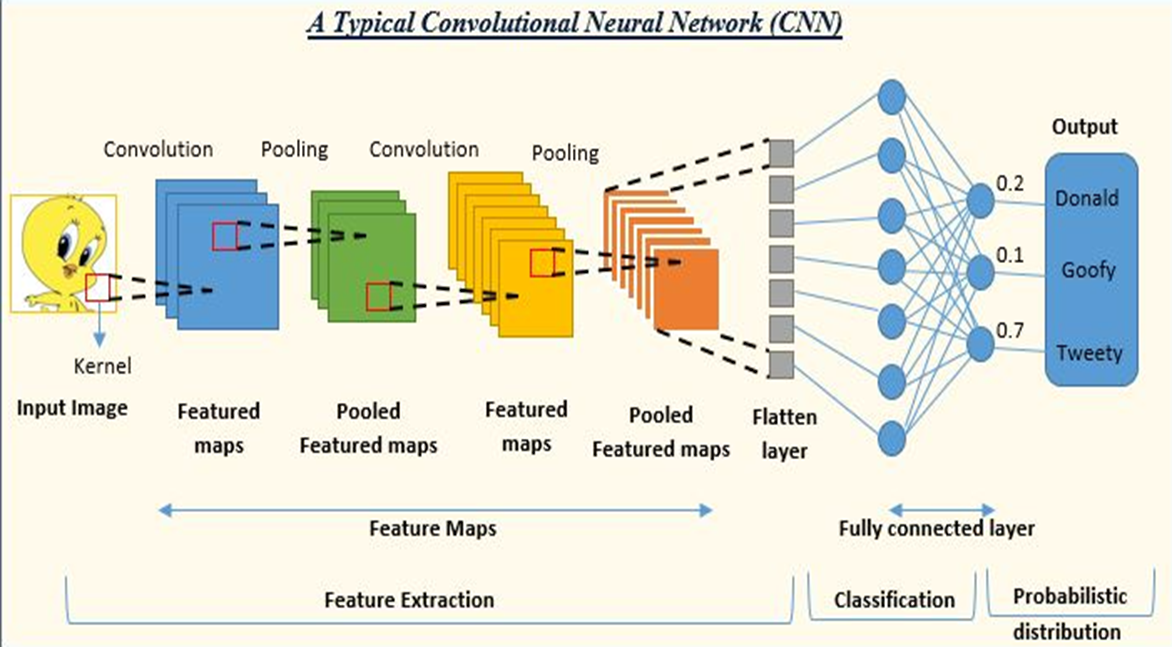
\includegraphics[width=0.9\linewidth]{Images/cnnarchi.png}
    \caption{Kiến trúc điển hình của CNN}
    \label{fig:enter-label}
\end{figure}

\begin{itemize}
    \item \textbf{Lớp Convolution (Conv):}
    \begin{itemize}
        \item Sử dụng bộ lọc (kernel) quét qua ảnh để phát hiện đặc trưng (ví dụ: cạnh, texture).
        \item Ví dụ: Kernel 3×3 với stride=1 và padding="same" giữ nguyên kích thước ảnh.
    \end{itemize}
    \item \textbf{Lớp Activation Function:} 
    \begin{itemize}
        \item ReLU (Rectified Linear Unit) là hàm kích hoạt phổ biến nhất, giúp mô hình hội tụ nhanh hơn.
        \item Sigmoid là một hàm kích hoạt phi tuyến có dạng chữ "S", biến đổi đầu vào thành khoảng giá trị từ 0 đến 1, thường được sử dụng trong các mô hình phân loại nhị phân để dự đoán xác suất.
    \end{itemize}
    \item \textbf{Lớp Pooling (Max/Average):}
    \begin{itemize}
        \item Giảm kích thước không gian (downsampling), tăng tính bất biến với nhiễu.
        \item Ví dụ: Max Pooling 2×2 giảm 50% kích thước ảnh.
    \end{itemize}
    \item \textbf{Lớp Fully Connected (FC):} Kết nối toàn bộ đặc trưng để phân loại (thường dùng ở cuối mô hình).
\end{itemize}
\subsubsection{Ưu điểm của CNN}
\begin{itemize}
    \item \textbf{Hiệu quả với dữ liệu ảnh:} Tận dụng tính chất cục bộ (local connectivity) và trọng số chia sẻ (shared weights), giảm overfitting.
    \item \textbf{Tiết kiệm tài nguyên:} Ít tham số hơn so với mạng DNN nhờ cơ chế convolution.
    \item \textbf{Khả năng mở rộng:} Dễ dàng kết hợp với các kiến trúc hiện đại (ResNet, Transformer).
\end{itemize}
\subsubsection{Ứng dụng điển hình}
\begin{itemize}
    \item \textbf{Nhận diện đối tượng:} Phát hiện khuôn mặt, chữ số viết tay (MNIST).
    \item \textbf{Phân đoạn ảnh y tế:} Xác định khối u trong ảnh MRI.
    \item \textbf{Xử lý video:} Theo dõi chuyển động trong camera an ninh.
\end{itemize}
\subsubsection{Biến thể nâng cao của CNN}
\begin{itemize}
    \item \textbf{ResNet:} Giải quyết vấn đề vanishing gradient bằng kết nối tắt (skip connection).
    \item \textbf{MobileNet:} Tối ưu cho thiết bị di động nhờ convolution tách rời (depthwise separable conv).
    \item \textbf{EfficientNet:} Cân bằng giữa độ chính xác và kích thước mô hình qua scaling coefficient.
\end{itemize}

\subsection{Xây dựng mô hình}
\textbf{Nền tảng thiết kế:} 
Mô hình CNN được đề xuất kế thừa các nguyên tắc cốt lõi từ AlexNet (khả năng trích xuất đặc trưng đa lớp với kernel lớn) và LeNet (kiến trúc đơn giản, phù hợp phần cứng), đồng thời để tối ưu hóa cho triển khai trên FPGA ta cần phải thay đổi mô hình theo các kỹ thuật sau.
\begin{figure}[H]
    \centering
    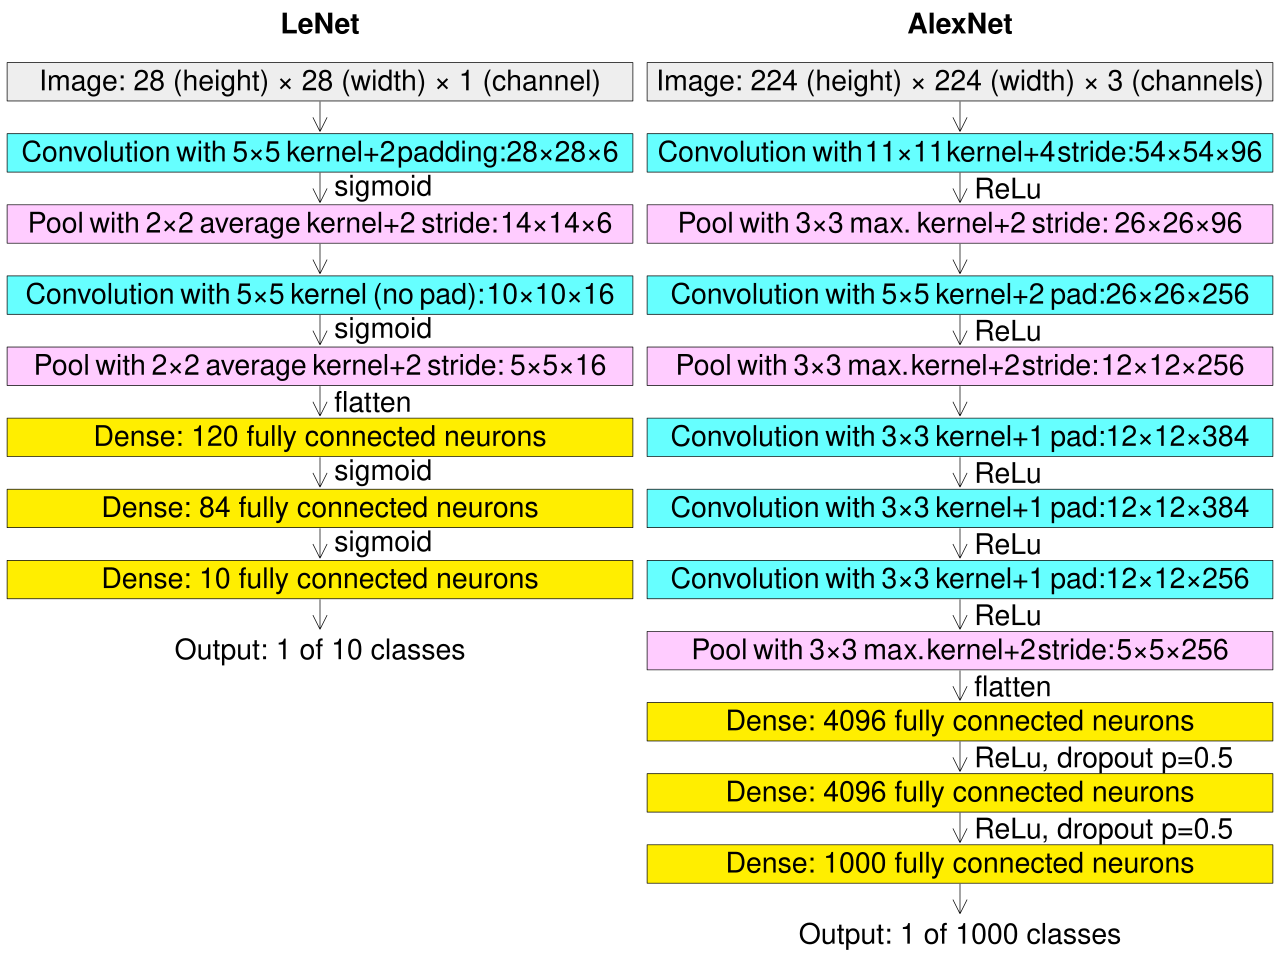
\includegraphics[width=0.75\linewidth]{Images/alexlenet.png}
    \caption{Cấu trúc mô hình LeNet và AlexNet}
    \label{fig:enter-label}
\end{figure}

\subsubsection{Xử lý đầu vào thực tế}
Tích hợp tiền xử lý ảnh trực tiếp trên FPGA (grayscale, resize về 28x28 như LeNet) để giảm latency. Và cũng phù hợp với Dataset MNIST đồ án này sử dụng để đào tạo mạng CNN.
\subsubsection{Thay thế và giảm bớt lớp fully connect}
Các mạng phổ biến cho nhận dạng chữ số viết tay bao gồm LeNet và AlexNet, những mạng này thường được sử dụng cho các tác vụ phân loại hình ảnh. Tuy nhiên, trong triển khai phần cứng, các mạng này có thể không phù hợp lắm do số lượng tham số lớn, vì vậy cần phải điều chỉnh các mạng này. Đặc biệt, các lớp fully connected yêu cầu rất nhiều trọng số (weight) và các bộ DSP. Ví dụ nếu số input fully connect là 100, output là 10 thì tổng số trọng số là 100x10 và 10 bias cho lớp fully connect này. 
\begin{figure}
    \centering
    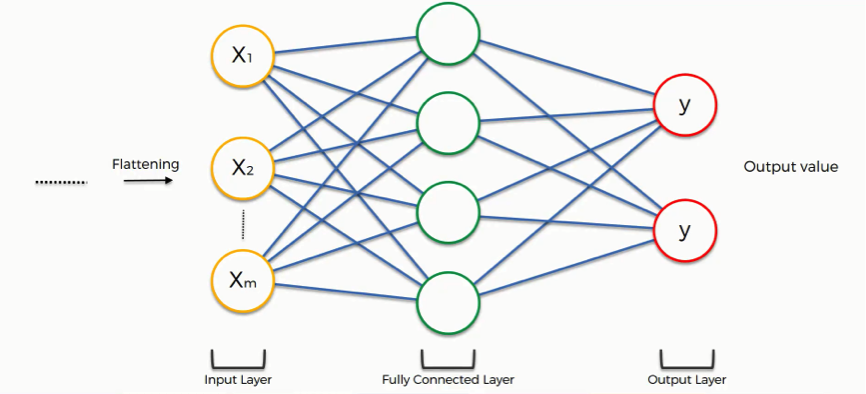
\includegraphics[width=0.75\linewidth]{Images/fullyconn.png}
    \caption{Fully connect}
    \label{fig:enter-label}
\end{figure}
Do đó để tiết kiệm tài nguyên triển khai, chúng ta cần giảm bớt trọng số của các lớp này. Một phương pháp phổ biến là sử dụng global max pooling để thay thế một phần trọng số của các lớp fully connected.
\begin{figure}[H]
    \centering
    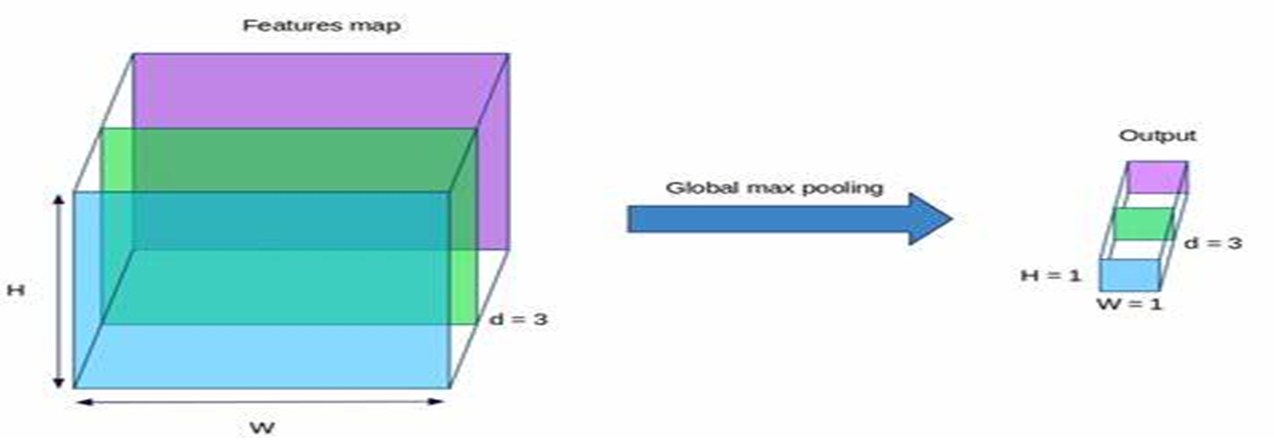
\includegraphics[width=0.75\linewidth]{Images/gmp.png}
    \caption{Global max pooling}
    \label{fig:enter-label}
\end{figure}
\subsubsection{Sử dùng hàm kích hoạt ReLU}
Hàm kích hoạt \textbf{ReLU} (Rectified Linear Unit) được định nghĩa:
\begin{equation}
    \text{ReLU}(x) = \max(0, x)
\end{equation}
\textbf{Lợi ích:}
\begin{itemize}
    \item \textbf{Tính toán hiệu quả}:
    \begin{equation}
        \text{Phép toán} \Rightarrow \begin{cases} 
        0 & \text{nếu } x < 0 \\
        x & \text{nếu } x \geq 0 
        \end{cases}
    \end{equation}
    Chỉ cần bộ so sánh (comparator) và multiplexer đơn giản
    
    \item \textbf{Tiết kiệm tài nguyên}:
    \begin{itemize}
        \item Không dùng phép nhân/phép chia phức tạp
        \item Chiếm ít LUTs (Look-Up Tables) trên FPGA
    \end{itemize}
    
    \item \textbf{Tận dụng pipeline}:
    $
        \text{Throughput} \uparrow \text{ nhờ latency thấp}
    $
    
    \item \textbf{Tương thích lượng tử hóa}:
    $
        \text{ReLU quan hệ tuyến tính} \Rightarrow \text{dễ dàng INT8/BNN hóa}
    $

\end{itemize}

\subsubsection{Binary Convolution (Tích chập nhị phân)}
Binary Weight Networks lượng tử hóa trọng số thành 2 giá trị $\{-1, +1\}$ nhưng giữ nguyên đầu vào full-precision. Công thức cơ bản:

\begin{equation}
    \mathbf{Y} = \mathbf{X} \ast \text{sign}(\mathbf{W})
\end{equation}

\noindent với:
\begin{itemize}
    \item $\mathbf{X}$: Đầu vào full-precision (float32)
    \item $\mathbf{W}$: Trọng số nhị phân hóa qua hàm $\text{sign}(\cdot)$
    \item $\ast$: Phép tích chập thông thường
\end{itemize}

\textbf{Quá trình nhị phân hóa}
\begin{equation}
    \text{sign}(W_{ij}) = \begin{cases} 
        +1 & \text{nếu } W_{ij} \geq 0 \\
        -1 & \text{nếu } W_{ij} < 0 
    \end{cases}
\end{equation}

\noindent Kèm theo scaling factor $\alpha$ để bù sai số:
\begin{equation}
    \alpha = \frac{1}{n} \|\mathbf{W}\|_1 = \frac{1}{n} \sum_{i,j} |W_{ij}|
\end{equation}

\textbf{Ưu điểm phần cứng}
\begin{itemize}
    \item \textbf{Tiết kiệm bộ nhớ}: Giảm 32x so với float32
    \item \textbf{Tối ưu phép nhân}: 
    \begin{equation}
        x \times \text{sign}(w) = \begin{cases} 
            +x & \text{nếu } w \geq 0 \\
            -x & \text{nếu } w < 0 
        \end{cases}
    \end{equation}
    \item Triển khai trên FPGA chỉ cần:
    \begin{itemize}
        \item Multiplexer chọn giữa $+x$ và $-x$
        \item Không cần DSP blocks cho phép nhân
    \end{itemize}
\end{itemize}

\textbf{Triển khai trên FPGA}
\begin{verbatim}
module binary_weight_layer (
    input [31:0] input_data,
    input binary_weight,
    output reg [31:0] result
);
    always @(*) begin
        result = (binary_weight == 1'b1) ? input_data : -input_data;
    end
endmodule
\end{verbatim}

\textbf{So sánh với Full-Precision và Xnor-net}
\begin{table}[h]
    \centering
    \begin{tabular}{|l|c|c|c|}
    \hline
    \textbf{Thông số} & \textbf{Full-Precision} & \textbf{Binary Weight} & \textbf{XNOR-Net} \\ \hline
    Bộ nhớ trọng số & 32 bit/parameter & 1 bit/parameter & 1 bit/parameter \\ \hline
    Bộ nhớ activations & 32 bit & 32 bit & 1 bit \\ \hline
    Phép toán nhân & Float multiplier & MUX + inverter & XNOR + popcount \\ \hline
    Tốc độ (FPGA) & 1x & 2.7x & 58x \\ \hline
    Độ chính xác & Baseline & Giảm 1-3\% & Giảm 8-12\% \\ \hline
    Năng lượng tiêu thụ & 100\% & 35\% & 12\% \\ \hline
    Scaling factor & Không cần & $\alpha$ cho weights & $\alpha$, $\beta$ cho activations \\ \hline
    Triển khai phần cứng & DSP blocks & LUTs + MUX & Pure LUTs \\ \hline
    \end{tabular}
\end{table}
\begin{figure}[H]
    \centering
    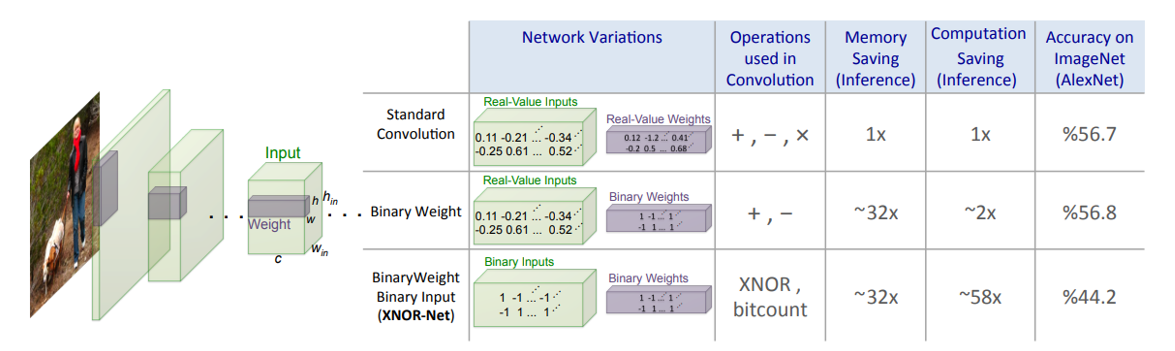
\includegraphics[width=0.9\linewidth]{Images/comparebinaryw.png}
    \caption{So sánh các phương pháp convolution}
    \label{fig:enter-label}
\end{figure}

\textbf{Xây dựng lớp Binary Convolution trên Tensorflow}
Vì Tensorflow không hỗ trợ sẵn nên ta cần phải dựa vào cấu trúc lớp Convolution mặc định để xây dựng lớp Binary Convolution. Với quá trình \textit{Forward} của lớp Convolution mặc định ta sẽ nhị phân hóa trọng số bằng cách sử dụng hàm \textit{tf.sign()}, giữ nguyên trọng số và \textit{Gradient} cho quá trình \textit{Backpropagation} để hội tụ nhanh hơn. 
\begin{lstlisting}[style=pythonstyle]
@tf.custom_gradient
def binarize(weights):
    """Function binarize weights with Straight-Through Estimator gradient"""
    def grad(dy, variables=None): 
        return dy  # Keep input gradient
    return tf.sign(weights), grad  # Binarize + custom gradient
\end{lstlisting}
\noindent\textbf{Giải thích:}
\begin{itemize}
    \item \texttt{@tf.custom\_gradient}: Decorator định nghĩa gradient tùy chỉnh
    \item \texttt{tf.sign(weights)}: Chuyển weights thành giá trị nhị phân $\{-1, 1\}$
    \item \texttt{grad(dy)}: Triển khai Straight-Through Estimator (STE) - truyền nguyên gradient đầu vào khi backpropagation
\end{itemize}

Với scaling-factor $\alpha$ để đơn giản phần lập trình ta đơn giản thay thế bằng cách thêm một lớp Batch Normalize sau lớp Binary Convolution. \\

Batch Normalization (BN) là kỹ thuật chuẩn hóa dữ liệu theo batch trong quá trình huấn luyện mạng neural, giúp ổn định và tăng tốc độ hội tụ.

\begin{equation}
    \hat{x}_i = \frac{x_i - \mu_B}{\sqrt{\sigma_B^2 + \epsilon}}
\end{equation}
\begin{equation}
    y_i = \gamma \hat{x}_i + \beta
\end{equation}


Trong đó:
\begin{itemize}
\item $\mu_B, \sigma_B^2$: Trung bình và phương sai của batch
\item $\gamma, \beta$: Tham số học được (scale và offset)
\item $\epsilon$: Hằng số tránh chia cho 0 (thường $10^{-5}$)
\end{itemize}
\textbf{Công dụng chính}
\begin{itemize}
    \item \textbf{Ổn định huấn luyện}: Giảm hiện tượng "internal covariate shift"
    \item \textbf{Hỗ trợ learning rate lớn}: Gradient ổn định hơn
    \item \textbf{Giảm phụ thuộc khởi tạo}: Ít nhạy cảm với giá trị ban đầu
    \item \textbf{Regularization ẩn}: Noise từ thống kê batch giảm overfitting
    \item \textbf{Tối ưu inference}: Sử dụng mean/variance cố định khi dự đoán
\end{itemize}

\subsection{Kết quả}
Từ cở sở trên ta xây dựng mô hình gồm 5 lớp Binary Convolution với sau mỗi lớp tích chập là khối Batch Normalize và Activation ReLU, 2 khối Max Pooling, 1 lớp Global Max Pooling và cuối cùng là 1 lớp Fully Connect.
\begin{figure}[H]
    \centering
    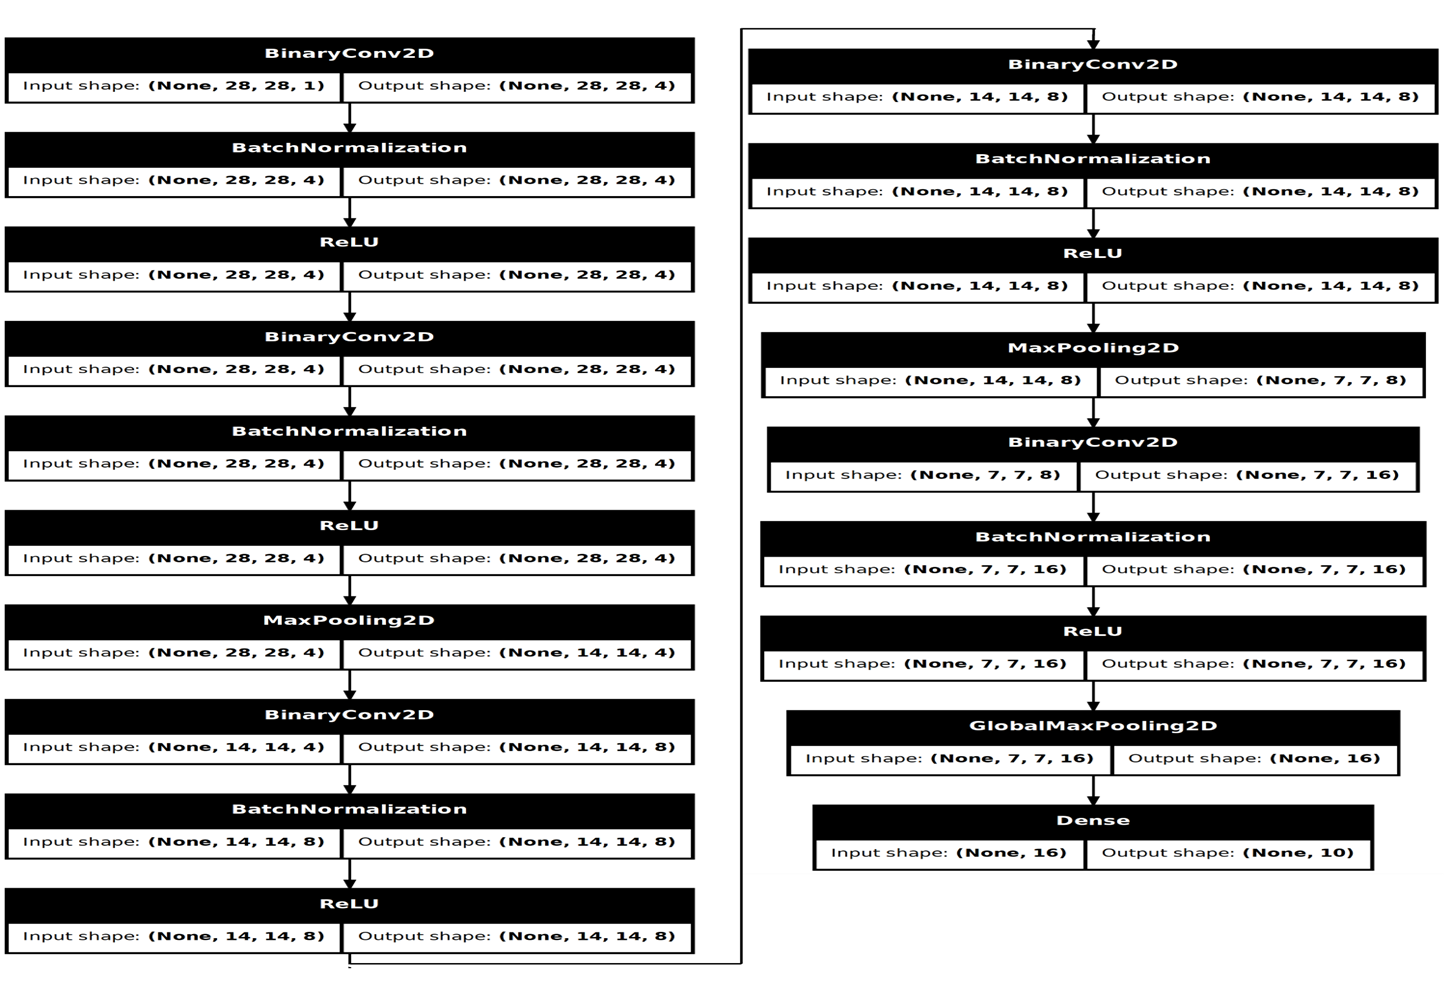
\includegraphics[width=1\linewidth]{Images/image.png}
    \caption{Model CNN}
    \label{fig:enter-label}
\end{figure}

\textbf{Kết quả training}
\begin{figure}[H]
    \centering
    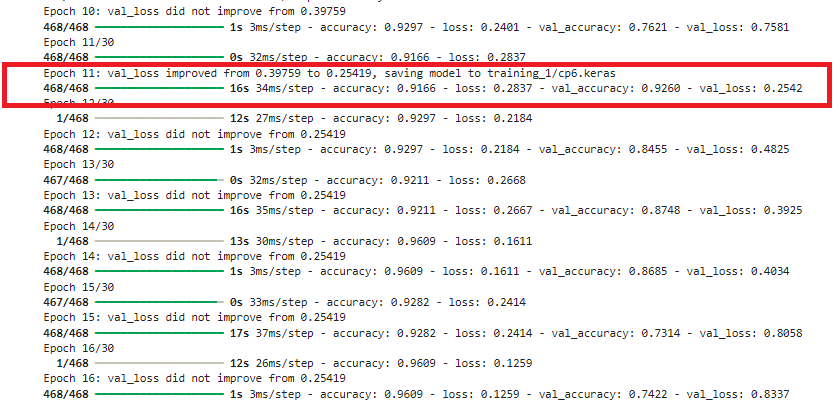
\includegraphics[width=0.9\linewidth]{Images/training.png}
    \caption{Kết quả training}
    \label{fig:enter-label}
\end{figure}
Quá trình training model sử dụng Adam optimizer với learning rate $10^{-4}$ có early stop ta có kết quả nhân diện đúng trên tập data \textit{Train} là $91.66\%$ loss $0.2873$ và kết quả trên tập data \textit{Evaluate} là $92.6\%$ loss $0.2542$
\begin{figure}[H]
    \centering
    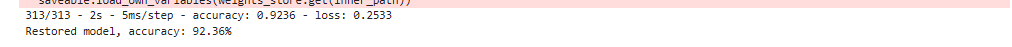
\includegraphics[width=0.9\linewidth]{Images/traintest.png}
    \caption{Kết quả test data MNIST}
    \label{fig:mnisttest}
\end{figure}
Kết quả test trên tập data \textit{Test} của MNIST có độ chính xác khoảng $92.36\%$.
\newpage
\section{THIẾT KẾ PHẦN CỨNG}
\subsection{Tổng quan hệ thống}
\subsubsection{Giới thiệu}
Hệ thống CNN (Convolutional Neural Network) được thiết kế trong tài liệu này tập trung vào việc phân tích ảnh xám và dự đoán chữ số từ 0 đến 9 dưới dạng mã BCD (Binary-Coded Decimal), kết hợp giữa kiến trúc phần cứng tối ưu và thuật toán học sâu. Mô-đun CNN áp dụng ý tưởng thiết kế hệ thống số về mô-đun điều khiển/xử lý dữ liệu, chia toàn bộ mạng nhận dạng thành hai khối chính:
\begin{itemize}
    \item \textbf{Khối điều khiển (máy trạng thái FSM)} Phát lệnh điều khiển dựa trên tín hiệu và trạng thái từ khối xử lý dữ liệu.
    \item  \textbf{Khối xử lý dữ liệu (Datapath)} Nhận lệnh từ khối điều khiển để thực hiện tính toán và phản hồi trạng thái hiện tại.
\end{itemize}

\subsubsection{Sơ đồ thiết kế phần cứng}
\begin{figure}[H]
    \centering
    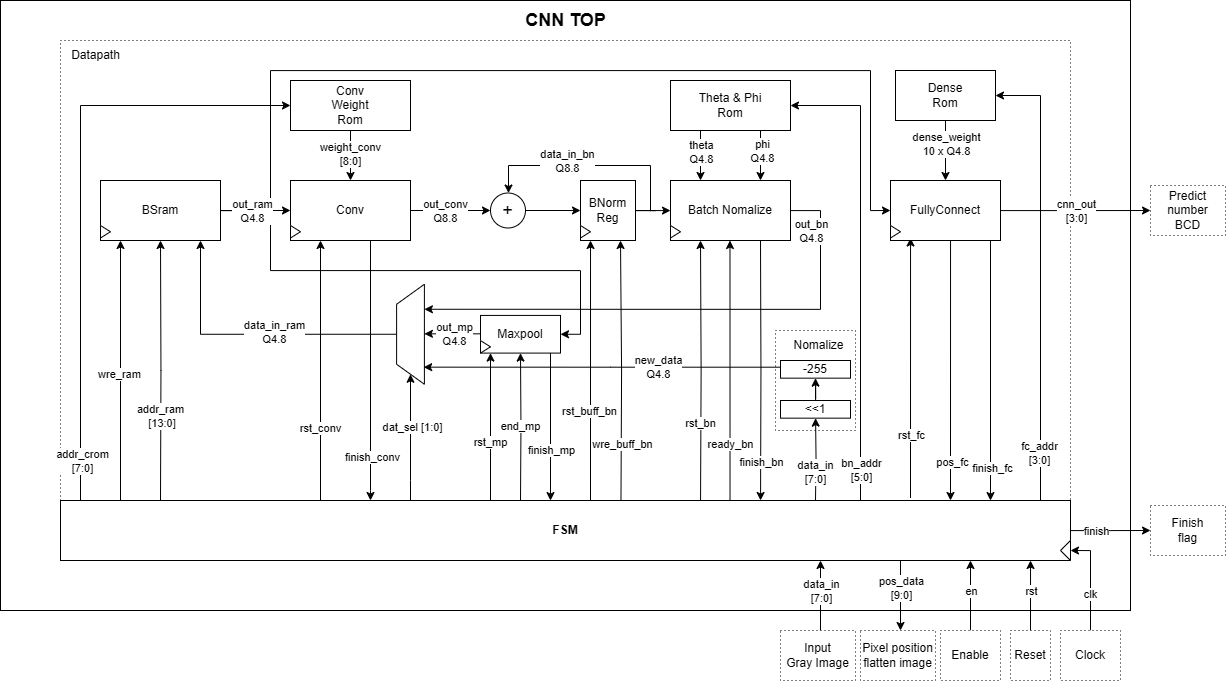
\includegraphics[angle=-90, width=0.75\linewidth]{Images/datapath_cnn.drawio.png}
    \caption{Sơ đồ thiết kế phần cứng khối CNN}
    \label{fig:tkpc}
\end{figure}


\subsubsection{Mục tiêu thiết kế}
\begin{itemize}
    \item \textbf{Xử lý ảnh hiệu quả:} Tiếp nhận đầu vào là điểm ảnh xám 8-bit, kết hợp theo dõi vị trí để tối ưu bộ nhớ.
    \item \textbf{Tối ưu tài nguyên:} Sử dụng định dạng dấu phẩy tĩnh (Q4.8, Q8.8) để cân bằng độ chính xác và chi phí tính toán. Việc sử dụng nhiều các khối chuẩn hóa giúp cho dữ liệu sau khi tính toán giao động từ $[-1; 1]$ do đó chọn địn dạng số có dấu Q4.8 với tầm từ $[-8; 7.99609375]$ lượng tử với độ phân giải $\frac{1}{256}$. Dữ liệu trung gian Q8.8 để dự phòng cho trường hợp ngõ vào của khối Batch Normalize là tổng tích chập nhiều \textit{Window} (Tối đa là 8 \textit{Window} với mô hình của đề tài) với nhau, ngoài ra Q8.8 còn sử dụng trong ruột của khối Fully Connect.
\end{itemize}

\subsubsection{Thông số kỹ thuật chính}

Thiết kế pipeline xử lý ảnh xám đầu vào qua 4 giai đoạn chính: Convolution → Batch Normalization → Max Pooling → Fully Connected.

\begin{itemize}
    \item \textbf{Định dạng dữ liệu:}
    \begin{itemize}
        \item Đầu vào: 8-bit grayscale + 10-bit vị trí (pos\_data[9:0]).
        \item Trung gian: Q4.8/Q8.8 fixed-point.
        \item Đầu ra: 4-bit BCD (cnn\_out[3:0])
    \end{itemize}

    \item \textbf{Bộ nhớ:}
    \begin{itemize}
        \item BRAM 14-bit address (addr\_ram[13:0])
        \item 3 ROM chứa:
        \begin{itemize}
            \item Conv weights (9-bit)
            \item Theta/Phi params (Q4.8) (Đề cập sau)
            \item Dense layer weights (Q4.8)
        \end{itemize}
    \end{itemize}

\end{itemize}

\subsubsection{Đặc Điểm Nổi Bật}
\begin{itemize}
    \item \textbf{Kiến trúc phần cứng rõ ràng:} ách biệt khối xử lý (Convolution, BN, Pooling, FC) và điều khiển (FSM), đồng bộ qua các tín hiệu \textit{finish} và \textit{rst}.
    \item \textbf{Bộ nhớ chuyên biệt:} ROM lưu trọng số tích chập (9-bit) và tham số chuẩn hóa (Q4.8), BRAM lưu dữ liệu trung gian với địa chỉ 14-bit.
    \item \textbf{Đầu ra linh hoạt:} Kết quả dự đoán 4-bit BCD, phù hợp với các hệ thống nhúng hoặc giao tiếp vi điều khiển.
\end{itemize}

\subsection{Khối tích chập (Binary Convolution)}
\subsubsection{Ý Tưởng Thiết Kế}
\begin{itemize}
    \item Thiết kế một bộ tích chập (convolution unit) tối ưu cho xử lý tín hiệu số với:
    \begin{itemize}
        \item Đầu vào dạng fixed-point Q4.8 (12-bit)
        \item Đầu ra dạng Q8.8 (16-bit)
        \item Hỗ trợ kernel 3x3 (9 trọng số)
    \end{itemize}
    \item Kết hợp 2 module chính:
    \begin{itemize}
        \item \textit{SIPO19:} Chuyển đổi serial-to-parallel 1 to 9 cho từng bit dữ liệu
        \item \textit{conv:} Thực hiện phép tích chập bằng cách ghép 12 bộ SIPO19 độc lập và thực hiện phép cộng trừ dựa theo trọng số nhị phân.
    \end{itemize}
    \begin{figure}[H]
        \centering
        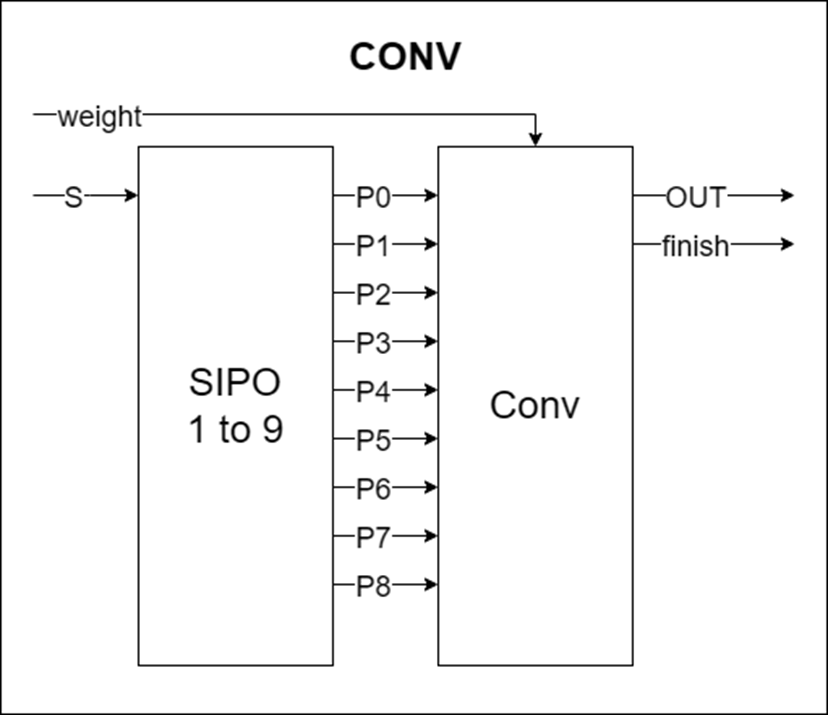
\includegraphics[width=0.75\linewidth]{Images/conv.png}
        \caption{Sơ đồ khối Binary Conv}
        \label{fig:enter-label}
    \end{figure}
    \item Sử dụng counter 4-bit để điều khiển luồng dữ liệu.
    \item Triển khai phép nhân qua thao tác XOR và cộng đơn giản. 
    \begin{verbatim}
        d_w[i] = (n_data[i]^{12{w[i]}})+{11'b0,w[i]}
    \end{verbatim}
\end{itemize}


\subsubsection{Thiết kế khối SIPO19}
\begin{verbatim}
    module SIPO19 (
    input clk, reset, serial_in, shift,
    output reg [8:0] parallel_out
    );
\end{verbatim}
\begin{itemize}
    \item Chức năng: 
    \begin{itemize}
        \item Dịch 9 bit nối tiếp → song song
        \item Giữ kết quả ở \textit{parallel\_out} khi \textit{shift=1}
    \end{itemize}
    \item Đặc điểm thiết kế:
    \begin{itemize}
        \item Thanh ghi 9-bit \textit{shift\_registe}r dịch trái mỗi chu kỳ clock
        \item Reset đồng bộ xóa cả thanh ghi và đầu ra
    \end{itemize}
\end{itemize}

\subsubsection{Thiết kế khối Conv}
\begin{table}[h]
\centering
\caption{Module Binary Convolution Signal Definitions}
\label{tab:signals}
\begin{tabular}{llll}
\toprule
\textbf{Signal Name} & \textbf{Direction} & \textbf{Width} & \textbf{Description} \\
\midrule
clk & Input & 1 & System clock \\
rst & Input & 1 & Active-high reset \\
en\_conv & Input & 1 & Convolution enable \\
data\_in & Input & 12 & Input data (Q4.8 format) \\
w & Input & 9 & Weight vector (0=add, 1=subtract) \\
finish & Output & 1 & Operation completion flag \\
out & Output & 16 & Result (Q8.8 format) \\
\bottomrule
\end{tabular}
\end{table}


\begin{itemize}
    \item Cơ chế hoạt động: 
    \begin{itemize}
        \item Giai đoạn load dữ liệu:
        \begin{itemize}
            \item 12 SIPO19 thu nhận từng bit của \textit{data\_in} khi \textit{sync=1}
            \item Mỗi SIPO19 tạo 9 bản sao song song của 1 bit dữ liệu
        \end{itemize}
        \item Giai đoạn tính toán:
        \begin{itemize}
            \item Tạo 9 phiên bản dữ liệu đã chuẩn hóa (\textit{d\_w[0:8]})
            \item Tính tổng có dấu với sign extension (bit mở rộng dấu)
        \end{itemize}
        \item Giai đoạn hoàn tất conv: Counter đếm đến 10 chu kỳ → báo \textit{finish}
    \end{itemize}
    \item Phép Toán Tích Chập
    \begin{itemize}
        \item Cơ chế nhân nhị phân: Với mỗi trọng số \textit{w[i]}
        \begin{itemize}
            \item Nếu \textit{w[i]=1}: Thực hiện phép đảo bit và cộng 1 (bù 2)
            \item Nếu \textit{w[i]=0}: Giữ nguyên giá trị
        \end{itemize}
        \item Mở rộng dấu 4 bit trước khi tính tổng (từ 12-bit → 16-bit)
    \end{itemize}
\end{itemize}


\subsubsection{Kiểm Thử \& Xác Minh}
\begin{table}[h]
\centering
\caption{Binary Convolution Verification Plan Table}
\begin{tabular}{>{\bfseries}p{2.5cm}p{4cm}p{4cm}p{3cm}}
\toprule
\textbf{Test Category} & \textbf{Test Case} & \textbf{Verification Method} & \textbf{Expected Result} \\
\midrule
Reset Verification & Power-on reset & Assert reset, then release & All registers cleared, outputs zero \\
\hline
SIPO Functionality & Serial data shifting & Input known pattern, verify parallel output & Correct parallel output after 9 cycles \\
\hline
Basic Convolution & All weights=0 (pure add) & Input fixed value, check output & Output = 9 × input \\
\hline
Basic Convolution & All weights=1 (pure subtract) & Input fixed value, check output & Output = -9 × input \\
\hline
Mixed Operation & Alternating weights & Input fixed value, mixed weights & Correct weighted sum \\
\hline
Timing Control & Enable/disable during operation & Toggle en\_conv at various times & Proper operation only when enabled \\
\hline
Finish Signal & Operation completion & Monitor finish signal & Asserted after 10 cycles \\
\hline
Boundary Cases & Maximum input value & Input 12'h7FF & Correct saturated output \\
\hline
Boundary Cases & Minimum input value & Input 12'h800 & Correct negative output \\
\hline
Reset Recovery & Reset during operation & Assert reset mid-calculation & Immediate termination, outputs zero \\
\bottomrule
\end{tabular}
\end{table}

\begin{figure}[H]
    \centering
    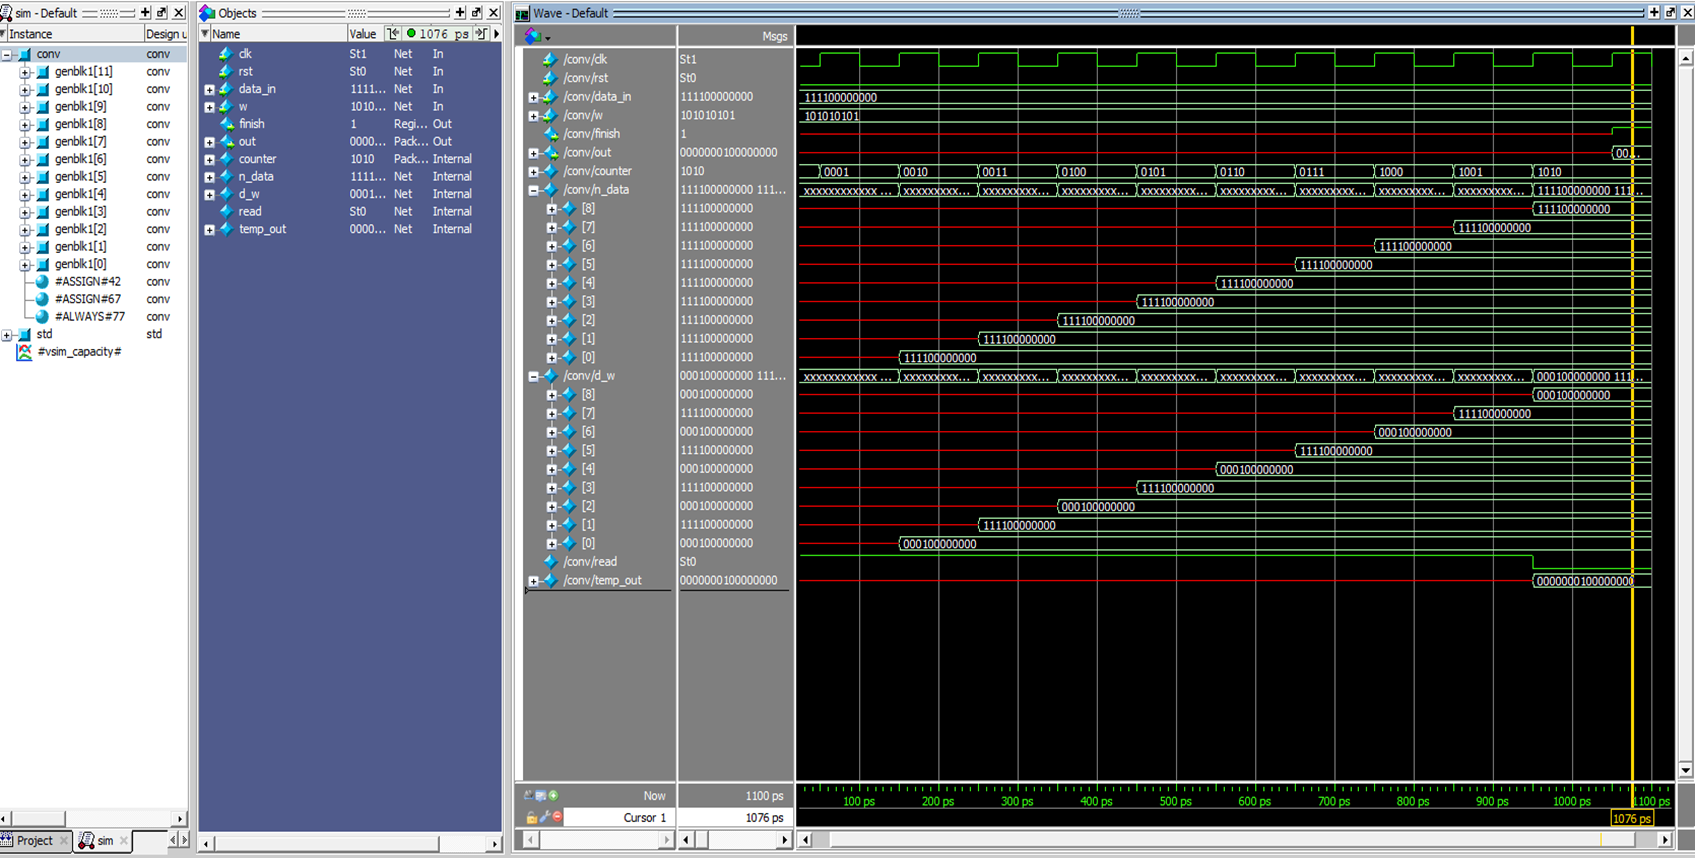
\includegraphics[width=0.9\linewidth]{Images/waveconv.png}
    \caption{Dạng sóng ngõ ra với testcase mixed weight với input bằng -1 (Q4.8)}
    \label{fig:enter-label}
\end{figure}
Quan sát thấy khí tín hiệu \textit{finish=1} kết quả ngõ ra bằng 1 (Q8.8) do ngõ vào cố định bằng -1 và với $weight=9'b101010101$ sẽ thực hiện 5 phép trừ và 4 phép cộng kết quả bằng 1 là chính xác. \\

VIết code testbench và sử dụng chức năng monitor của Modelsim để kiểm tra các testcase còn lại.
\begin{figure}[H]
    \centering
    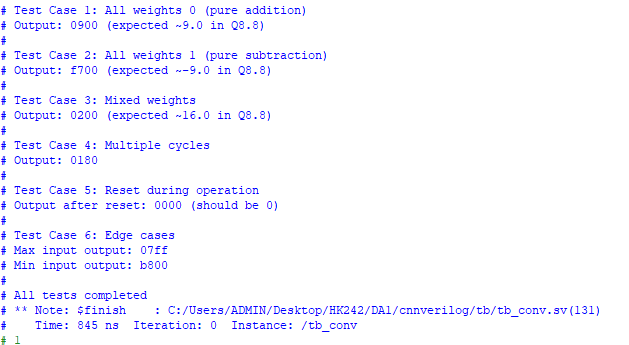
\includegraphics[width=0.75\linewidth]{Images/convtestcase.png}
    \caption{Testbench Conv}
    \label{fig:enter-label}
\end{figure}

\subsubsection{Synthesize}
Sử dụng phần mềm Gowin FPGA Designer để chạy synthesis ta có kết quả Netlist như hình \ref{fig:convsynth}.
\begin{figure}[H]
    \centering
    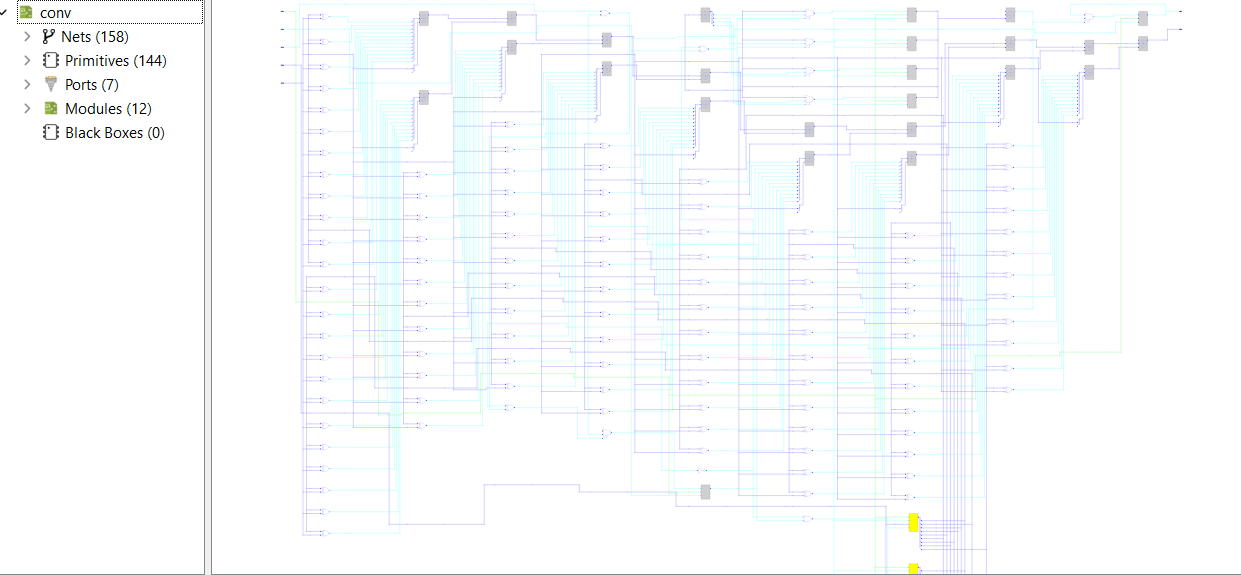
\includegraphics[width=0.75\linewidth]{Images/convsynth.png}
    \caption{Kết quả netlist synthesis khối Conv}
    \label{fig:convsynth}
\end{figure}

Ta có được báo cáo tài nguyên sử dụng và timing như sau.
\begin{table}[h]
\centering
\caption{Báo các sử dụng tài nguyên FPGA cho khối Conv}
\label{tab:resource_usage}
\begin{tabular}{
    l
    S[table-format=3.0]
    @{\hspace{1em}}
    S[table-format=4.0]
    S[table-format=1.1]
}
\toprule
\multirow{2}{*}{\textbf{Tài nguyên}} & 
\multicolumn{2}{c}{\textbf{Sử dụng/Tổng}} & 
\multirow{2}{*}{\textbf{Utilization}} \\
& \multicolumn{2}{c}{(đơn vị)} & \\
\midrule
Logic & 335 & (189 LUT, 128 ALU, 3 RAM16) / 8640 & 4.0\% \\
\hline
Register & \multicolumn{2}{l}{105 / 6693} & 2.0\% \\
\quad $\bullet$ Register as Latch & \multicolumn{2}{l}{0 / 6693} & 0.0\% \\
\quad $\bullet$ Register as FF & \multicolumn{2}{l}{105 / 6693} & 2.0\% \\
\hline
BSRAM & \multicolumn{2}{l}{0 / 26} & 0.0\% \\
\bottomrule
\end{tabular}

\vspace{0.5em}
\end{table}

\begin{figure}[H]
    \centering
    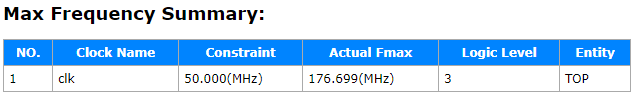
\includegraphics[width=0.9\linewidth]{Images/timingconv.png}
    \caption{Báo cáo timing khối Conv}
    \label{fig:enter-label}
\end{figure}

\subsection{Khối chuẩn hóa batch (Batch Nomalize)}
\subsubsection{Ý Tưởng Thiết Kế}
Nhắc lại phương trình tính Batch Normalize, mối quan hệ vào ra của dữ liệu được thể hiện qua công thức:
\begin{equation}
y_i = \gamma\frac{x_i-\mu}{\sqrt{\sigma^2}} + \beta
\end{equation}
Ta thấy khối này sử dụng 4 thông số trọng số, để giảm khói lượng tính toán và lưu trữ ta đơn giản phương trình như sau:
\begin{equation}
y_i = \gamma\frac{x_i-\mu}{\sqrt{\sigma^2}} + \beta = \theta x_i + \phi
\end{equation}
với:
\begin{itemize}
    \item $\theta = \gamma/\sqrt{\sigma^2}$ (hệ số tỷ lệ)
    \item $\phi = -\mu\gamma/\sqrt{\sigma^2} + \beta$ (hệ số dịch chuyển)
\end{itemize}

Với 2 hệ số $\theta$ và $\phi$ sẽ được tính toán trước và lượng tử hóa về kiểu dữ liệu Q4.8 do dựa theo khảo sát thì hệ số $\theta$ luôn dương và bé hơn 1 và hệ số $\phi$ của mô hình nằm trong khoảng kiểu dữ liệu Q4.8.
\begin{figure}[H]
    \centering
    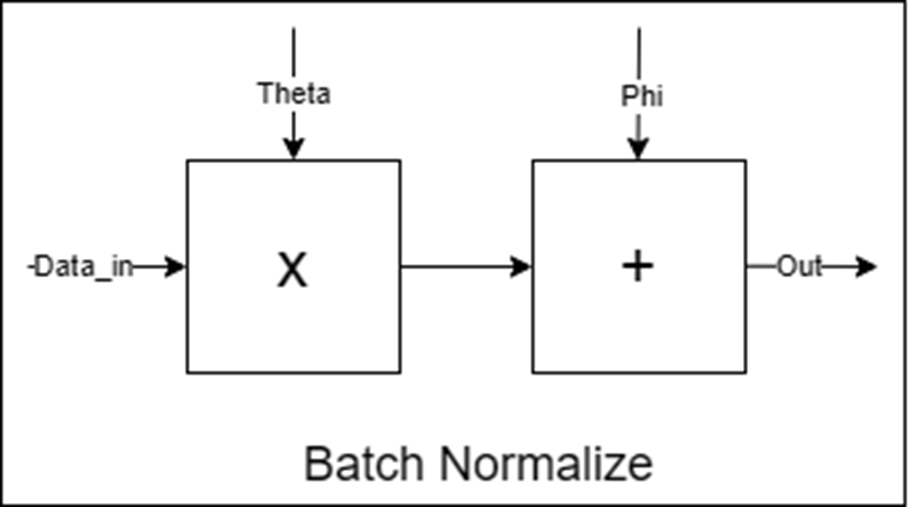
\includegraphics[width=0.5\linewidth]{Images/bnormblock.png}
    \caption{Sơ đồ khối Batch Nomalize}
    \label{fig:enter-label}
\end{figure}

\subsubsection{Thiết kế khối Batch Normalize}
\begin{table}[h]
\centering
\caption{Module BNORM Signal Definitions}
\label{tab:bnorm_signals}
\begin{tabular}{|>{\bfseries}l|l|l|l|}
\hline
\textbf{Signal Name} & \textbf{Direction} & \textbf{Width} & \textbf{Description} \\ \hline
clk      & Input  & 1  & System clock \\ \hline
rst      & Input  & 1  & Active-high reset \\ \hline
ready    & Input  & 1  & Data processing enable \\ \hline
data\_in & Input  & 16 & Input data (Q8.8 format) \\ \hline
theta    & Input  & 12 & Scale factor $\gamma/\sqrt{\sigma^2}$ \\ \hline
phi      & Input  & 12 & Shift factor $-\mu\gamma/\sqrt{\sigma^2} + \beta$ \\ \hline
finish   & Output & 1  & Operation completion flag \\ \hline
out      & Output & 12 & Result (Q4.8 format) \\ \hline
\end{tabular}
\end{table}

Bên trong khối này sẽ thực hiện tính toán ở kiểu dữ liệu Q8.8 sau đó cắt giảm 4 bit đầu để về kiểu dữ liệu Q4.8 và thực hiện luôn nhiệm vụ cuat lớp ReLU bằng cách kiểm tra bit MSB để quyết định kết quả ngõ ra. \\
\textbf{Các luồng tính toán chính}
\begin{itemize}
    \item Nhân với hệ số $\theta$:
    \begin{itemize}
        \item Mở rộng dấu ngõ vào 16-bit → 28-bit (Đảm bảo kết quả cho phép nhân có dấu 16-bit x 12-bit
        \item Nhân với $\theta$ (12-bit) sau khi mở rộng zero ($\theta$ luôn dương)
    \end{itemize}
    \item Cộng với hệ số $\phi$:
    \begin{itemize}
        \item Lấy 12 bit trung gian (bit 19-8) của kết quả nhân
        \item Cộng với hệ số dịch chuyển $\phi$
    \end{itemize}
    \item ReLU
    \begin{itemize}
        \item Phát hiện giá trị âm qua bit dấu (bit 11)
        \item Tự động cắt về 0 nếu âm (ReLU đơn giản)
    \end{itemize}
\end{itemize}
\textbf{Điều khiển trạng thái}
\begin{itemize}
    \item Tín hiệu \textit{finis}h được set sau 1 chu kỳ khi \textit{ready} active
    \item Reset đồng bộ thiết lập lại trạng thái
\end{itemize}

\subsubsection{Kiển thử \& Xác minh}

\begin{table}[h]
\centering
\caption{BNORM Module Verification Plan}
\label{tab:bnorm_verification}
\begin{tabular}{|l|l|l|}
\hline
\textbf{Test Category} & \textbf{Verification Method} & \textbf{Expected Result} \\ \hline
\multicolumn{3}{|c|}{\textbf{Reset Verification}} \\ \hline
Power-on reset & Assert reset, then release & All registers cleared, outputs zero \\ \hline
\multicolumn{3}{|c|}{\textbf{Basic Functionality}} \\ \hline
Identity transform & Set $\theta=1.0$, $\phi=0.0$ & Output = Input (Q4.8 scaled) \\ \hline
Scale only & Set $\theta=2.0$, $\phi=0.0$ & Output = 2 $\times$ Input \\ \hline
Shift only & Set $\theta=1.0$, $\phi=0.5$ & Output = Input + 0.5 \\ \hline
\multicolumn{3}{|c|}{\textbf{Boundary Cases}} \\ \hline
Max input value & Input 16'h7FFF (Q8.8) & Correct saturated output \\ \hline
Min input value & Input 16'h8000 (Q8.8) & Correct negative handling \\ \hline
Zero variance & Set $\theta=0.0$, $\phi=0.5$ & Output = 0.5 (constant) \\ \hline
\multicolumn{3}{|c|}{\textbf{Timing Control}} \\ \hline
Ready signal timing & Toggle ready during operation & Proper output only when ready=1 \\ \hline
Finish signal & Monitor finish signal & Asserted 2 cycles after ready \\ \hline
\multicolumn{3}{|c|}{\textbf{Reset Recovery}} \\ \hline
Mid-operation reset & Assert reset during calculation & Immediate termination, outputs zero \\ \hline
\end{tabular}
\end{table}

\begin{figure}[H]
    \centering
    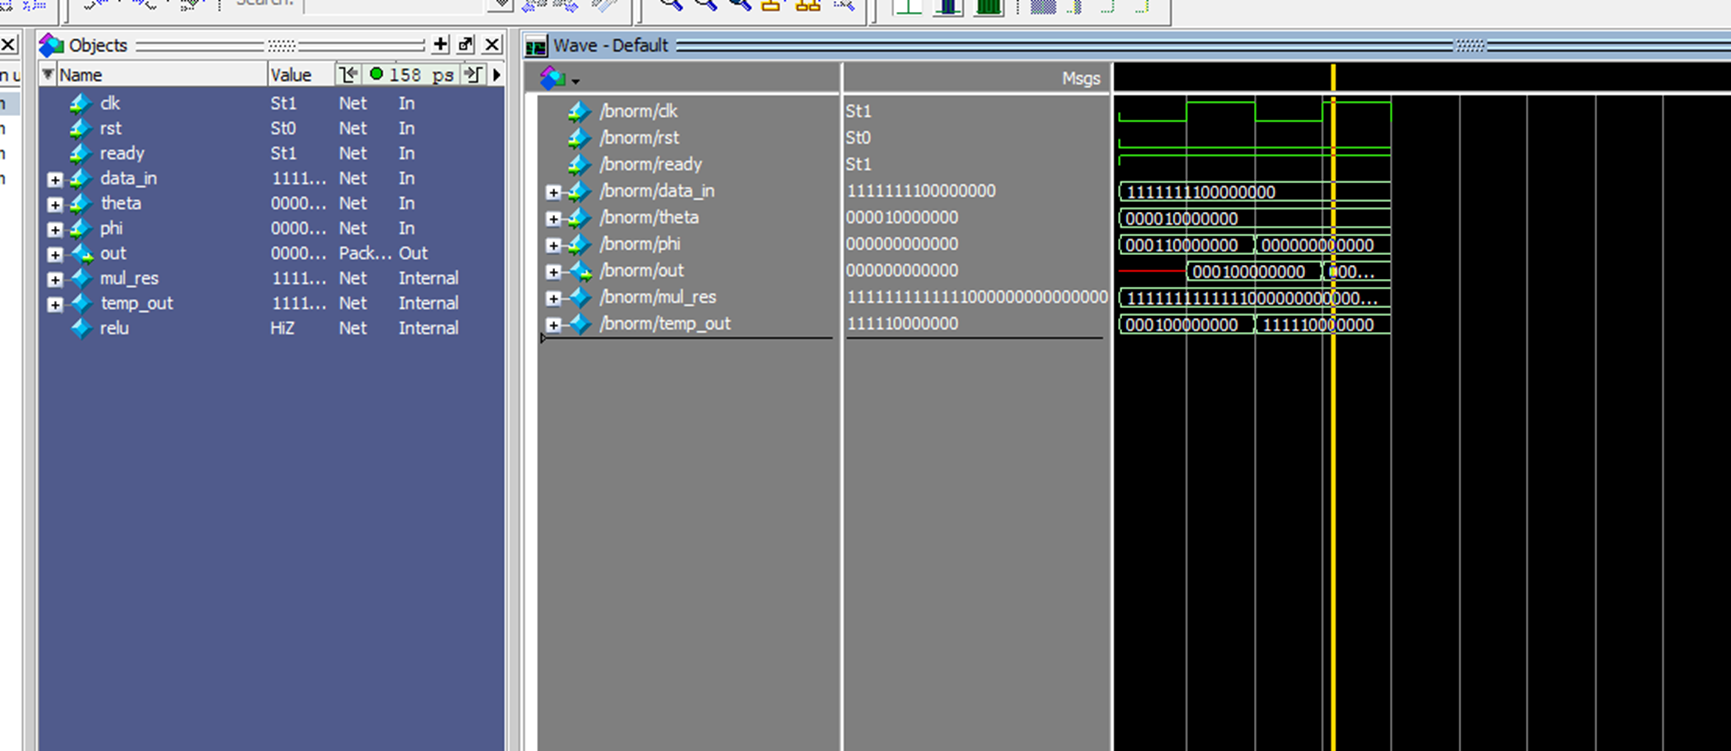
\includegraphics[width=0.75\linewidth]{Images/bnormtest.png}
    \caption{Dạng sóng ngõ ra với testcase Scale only với $\theta=1$ và ngõ vào bằng -1}
    \label{fig:enter-label}
\end{figure}
Quan sát khi tín hiệu \textit{finish=1} kết quả ngõ ra bằng -1 (Q4.8) do ngõ vào bằng -1 (Q8.8) với hệ số $\theta=1$ và $\phi=0$. \\
Viết code testbench và sử dụng chức năng monitor của Modelsim để kiểm tra các testcase
còn lại.

\begin{figure}[H]
    \centering
    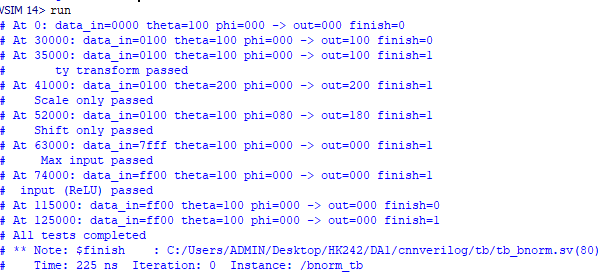
\includegraphics[width=0.75\linewidth]{Images/bnormtst.png}
    \caption{Testbench Bnorm}
    \label{fig:enter-label}
\end{figure}

\subsubsection{Synthesize}
Sử dụng phần mềm Gowin FPGA Designer để chạy synthesis ta có kết quả Netlist như hình \ref{fig:bnormsynth}.
\begin{figure}[H]
    \centering
    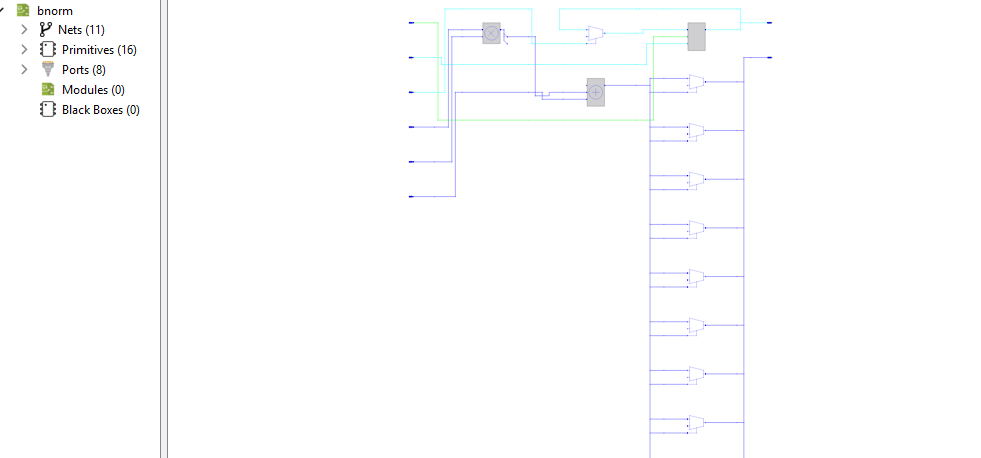
\includegraphics[width=0.75\linewidth]{Images/bnsynth.png}
    \caption{Kết quả netlist synthesis khối Bnorm}
    \label{fig:bnormsynth}
\end{figure}
Ta có được báo cáo tài nguyên sử dụng như sau.

\begin{table}[h]
\centering
\caption{Báo các sử dụng tài nguyên FPGA cho khối Bnorm}
\label{tab:resource_usage}
\begin{tabular}{
    l
    S[table-format=3.0]
    @{\hspace{1em}}
    S[table-format=4.0]
    S[table-format=1.1]
}
\toprule
\multirow{2}{*}{\textbf{Tài nguyên}} & 
\multicolumn{2}{c}{\textbf{Sử dụng/Tổng}} & 
\multirow{2}{*}{\textbf{Utilization}} \\
& \multicolumn{2}{c}{(đơn vị)} & \\
\midrule
Logic & 23 & (11 LUT, 12 ALU) / 8640 & <1.0\% \\
\hline
Register & \multicolumn{2}{l}{1 / 6693} & <1.0\% \\
\quad $\bullet$ Register as Latch & \multicolumn{2}{l}{0 / 6693} & 0.0\% \\
\quad $\bullet$ Register as FF & \multicolumn{2}{l}{1 / 6693} & <1.0\% \\
\hline
BSRAM & \multicolumn{2}{l}{0 / 26} & 0.0\% \\
\hline
DSP &  &  \\
\quad $\bullet$ MULT18X18 & \multicolumn{2}{l}{1} &  \\
\bottomrule
\end{tabular}

\vspace{0.5em}
\end{table}

\subsection{Khối Maxpool}
\subsubsection{Ý Tưởng Thiết Kế}
So sánh lần lượt các giá trị 12-bit (Q4.8) không cần để ý đến dấu. Nếu có giá trị lớn hơn giá trị temp thì sẽ thay thế temp bằng giá trị đó. Nếu có tín hiệu \textit{end} sẽ kết thúc quá trình so sánh và bật cờ $finish$. Có thể sử dụng khối này dùng cho quá trình Max pooling hoặc Global pooling.

\subsubsection{Thiết kế khối Maxpool}
\begin{table}[H]
\centering
\caption{Module MaxPool Signal Definitions}
\begin{tabular}{>{\ttfamily}l l l p{6cm}}
\toprule
\textbf{Signal Name} & \textbf{Direction} & \textbf{Width} & \textbf{Description} \\
\midrule
clk      & Input  & 1  & System clock \\
rst      & Input  & 1  & Active-high reset \\
data\_in & Input  & 12 & Input data (Q4.8 format) \\
end\_data & Input & 1  & End of input data flag \\
\midrule
finish   & Output & 1  & Operation completion flag \\
out      & Output & 12 & Max pooling result (Q4.8 format) \\
\bottomrule
\end{tabular}
\end{table}

Thiết kế khối Maxpool theo flow sau bằng ngôn ngữ verilog.
\begin{figure}[H]
    \centering
    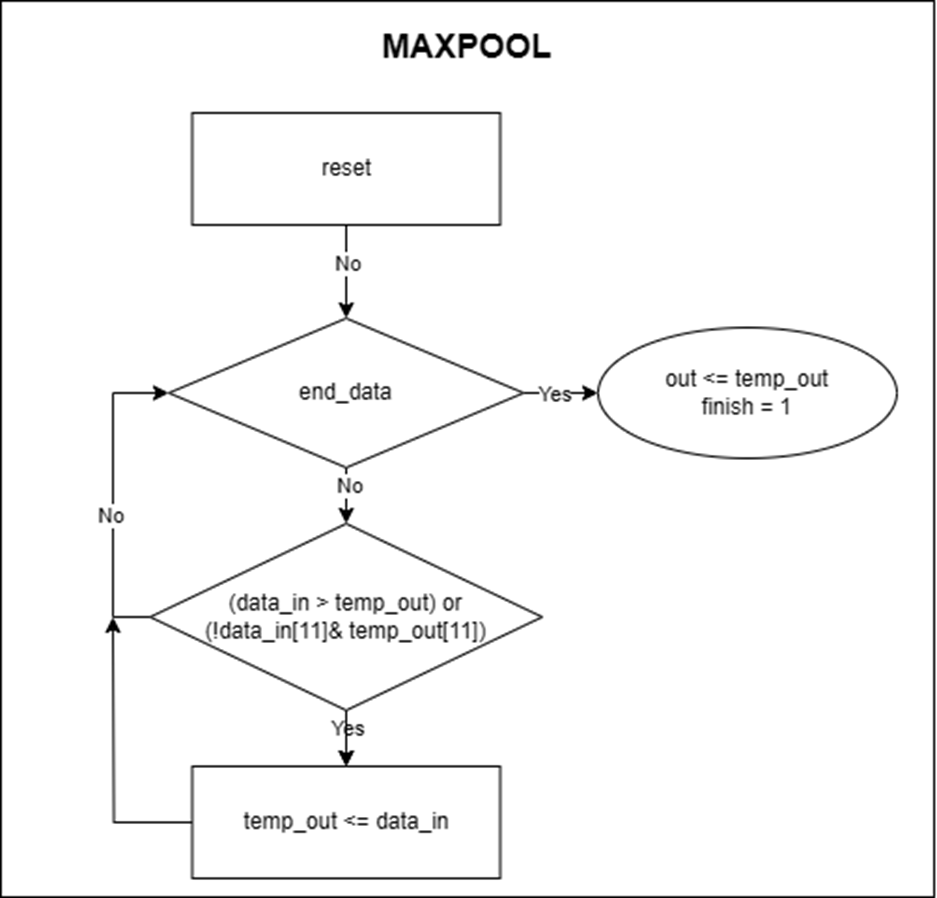
\includegraphics[width=0.75\linewidth]{Images/mpflow.png}
    \caption{Maxpool flow chart}
    \label{fig:enter-label}
\end{figure}

\subsubsection{Kiển thử \& Xác minh}

\begin{table}[h]
\centering
\caption{MaxPool Module Verification Plan}
\label{tab:maxpool_verification}
\begin{tabular}{|l|l|l|}
\hline
\textbf{Test Category} & \textbf{Verification Method} & \textbf{Expected Result} \\ \hline
\multicolumn{3}{|c|}{\textbf{Reset Verification}} \\ \hline
Power-on reset & Assert reset, then release & All registers cleared, outputs zero \\ \hline
Mid-operation reset & Assert reset during window processing & Immediate output reset to zero \\ \hline
\multicolumn{3}{|c|}{\textbf{Basic Functionality}} \\ \hline
Single 2x2 window & Input [1.0, 0.5, 1.5, 0.0] (Q4.8) & Output = 1.5 (max value) \\ \hline

Identical values & Input [0.8, 0.8, 0.8, 0.8] & Output = 0.8 (any duplicate accepted) \\ \hline
\multicolumn{3}{|c|}{\textbf{Boundary Cases}} \\ \hline
Max Q4.8 value & Input [7.996, 0.0, 0.0, 0.0] (16'h7FF) & Output = 7.996 \\ \hline

\multicolumn{3}{|c|}{\textbf{Timing Control}} \\ \hline
end\_data timing & Toggle end\_data during streaming & finish asserts 1 cycle after last window \\ \hline
Data starvation & Delay between input windows & Correct output timing with gaps \\ \hline
\multicolumn{3}{|c|}{\textbf{Error Cases}} \\ \hline
Incomplete window & Send 3 values then end\_data & Output remains zero (no false trigger) \\ \hline
\end{tabular}
\end{table}


\begin{figure}[H]
    \centering
    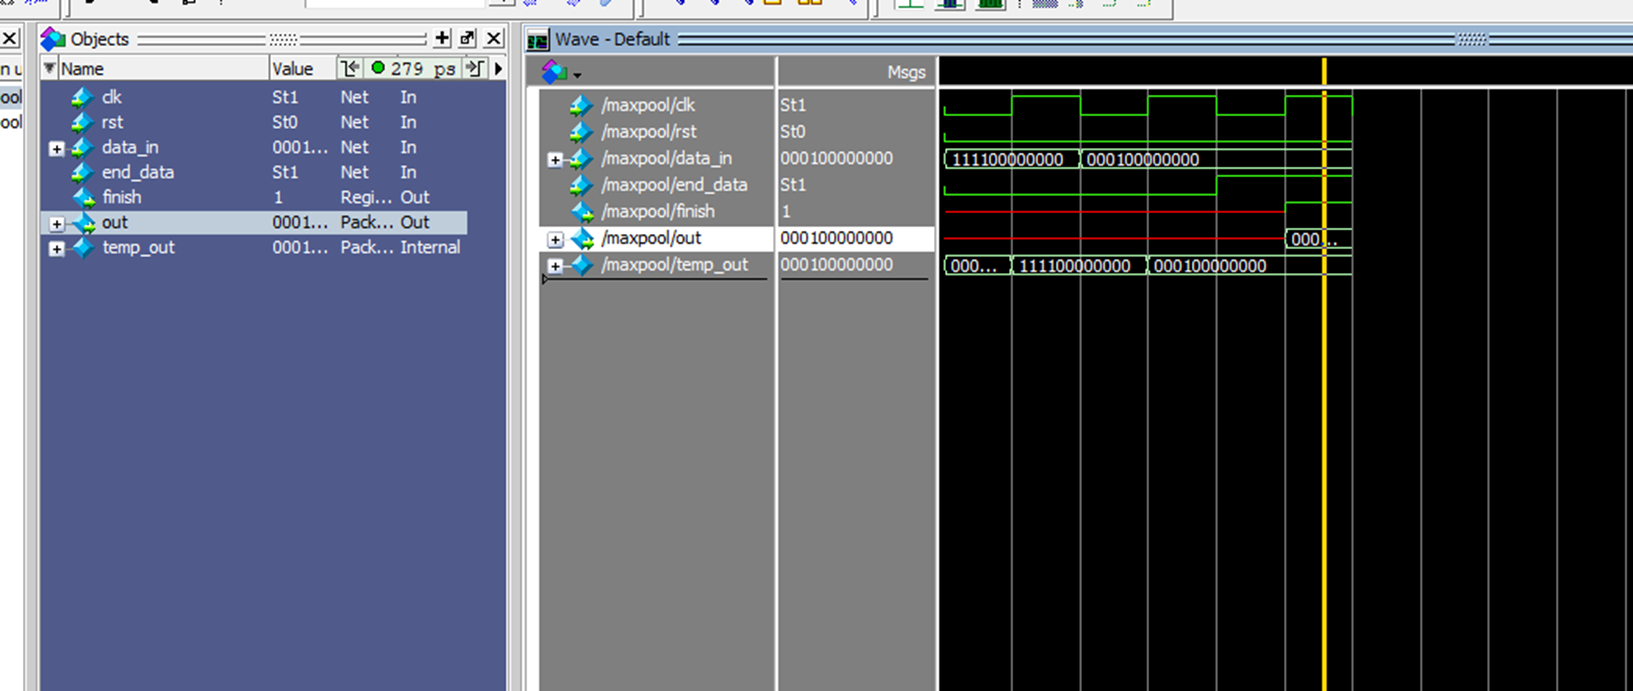
\includegraphics[width=0.9\linewidth]{Images/tbmp.png}
    \caption{Dạng sóng ngõ ra cho testcase chức năng chính khối maxpool}
    \label{fig:enter-label}
\end{figure}
Quan sát khi tín hiệu \textit{finish=1} kết quả ngõ ra bằng 1 (Q4.8) do ngõ vào lần lượt bằng -1 và 1 sau khi cờ \textit{end\_data} được bật sẽ bật cờ \textit{finish} và trả kết quả ngõ ra bằng 1. \\
Viết code testbench và kiểm tra dạng sóng các testcase còn lại.


\subsubsection{Synthesize}
Sử dụng phần mềm Gowin FPGA Designer để chạy synthesis ta có kết quả Netlist như hình \ref{fig:mpsynth}.
\begin{figure}[H]
    \centering
    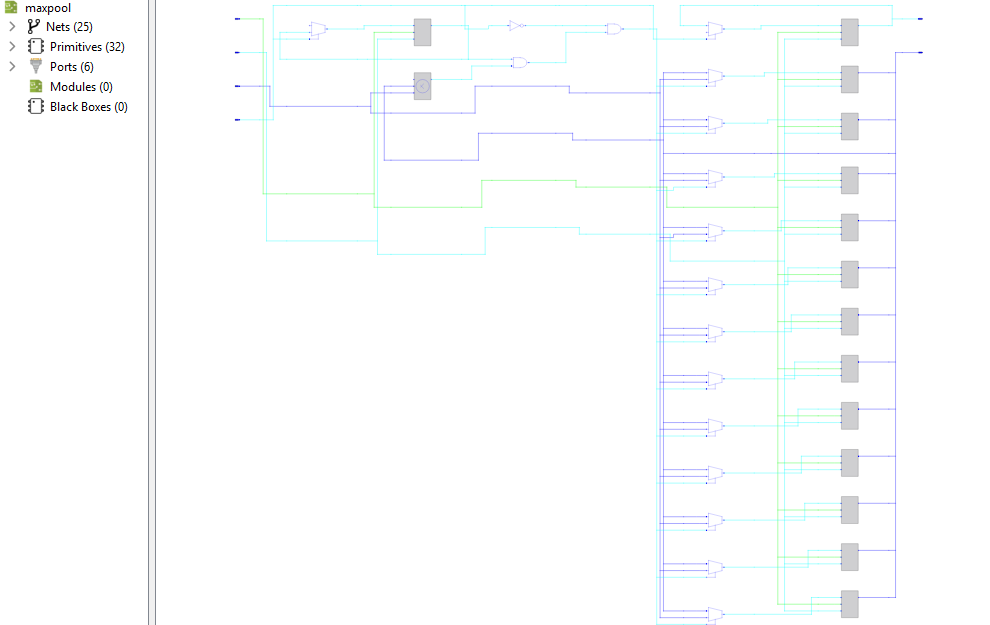
\includegraphics[width=0.75\linewidth]{Images/mpnet.png}
    \caption{Kết quả netlist synthesis khối Maxpool}
    \label{fig:mpsynth}
\end{figure}
Ta có được báo cáo tài nguyên sử dụng và timing như sau.

\begin{table}[H]
\centering
\caption{Báo các sử dụng tài nguyên FPGA cho khối Maxpool}
\label{tab:resource_usage}
\begin{tabular}{
    l
    S[table-format=3.0]
    @{\hspace{1em}}
    S[table-format=4.0]
    S[table-format=1.1]
}
\toprule
\multirow{2}{*}{\textbf{Tài nguyên}} & 
\multicolumn{2}{c}{\textbf{Sử dụng/Tổng}} & 
\multirow{2}{*}{\textbf{Utilization}} \\
& \multicolumn{2}{c}{(đơn vị)} & \\
\midrule
Logic & 14 & (2 LUT, 12 ALU) / 8640 & <1.0\% \\
\hline
Register & \multicolumn{2}{l}{14 / 6693} & <1.0\% \\
\quad $\bullet$ Register as Latch & \multicolumn{2}{l}{0 / 6693} & 0.0\% \\
\quad $\bullet$ Register as FF & \multicolumn{2}{l}{14 / 6693} & <1.0\% \\
\hline
BSRAM & \multicolumn{2}{l}{0 / 26} & 0.0\% \\
\hline
\bottomrule
\end{tabular}

\begin{figure}[H]
    \centering
    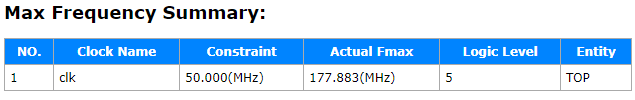
\includegraphics[width=0.9\linewidth]{Images/mptime.png}
    \caption{Báo cáo timing khối Maxpool}
    \label{fig:enter-label}
\end{figure}

\vspace{0.5em}
\end{table}

\subsection{Khối Fully Connect}
\subsubsection{Ý Tưởng Thiết Kế}
\begin{itemize}
    \item Thiết kế bộ fully connected layer tối ưu cho bài toán phân lớp 10 lớp:
    \begin{itemize}
        \item Đầu vào dạng fixed-point Q4.8 (12-bit)
        \item Trọng số dạng Q4.8 (12-bit)
        \item Đầu ra dạng one-hot 4-bit (10 lớp)
        \item Hỗ trợ batch size lên đến 16 mẫu (counter 4-bit)
    \end{itemize}
    
    \item Kết hợp 2 module chính:
    \begin{itemize}
        \item \textit{Multiply-Accumulate (MAC):} 10 bộ MAC song song cho 10 lớp đầu ra
        \item \textit{Max Tournament:} Cây so sánh 5 tầng để tìm lớp có giá trị lớn nhất
    \end{itemize}
    \begin{figure}[H]
        \centering
        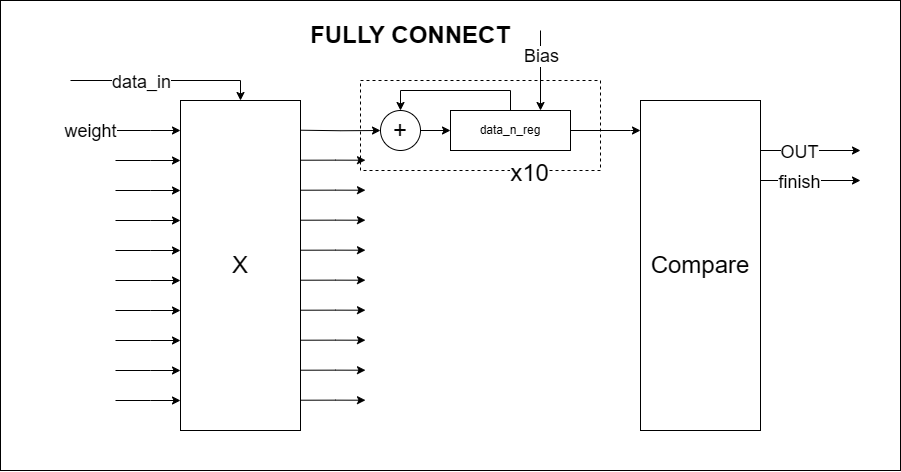
\includegraphics[width=0.8\linewidth]{Images/fc_arch.png}
        \caption{Sơ đồ khối FullyConnect với pipeline 3 giai đoạn}
        \label{fig:fc_arch}
    \end{figure}

    \begin{figure}[H]
        \centering
        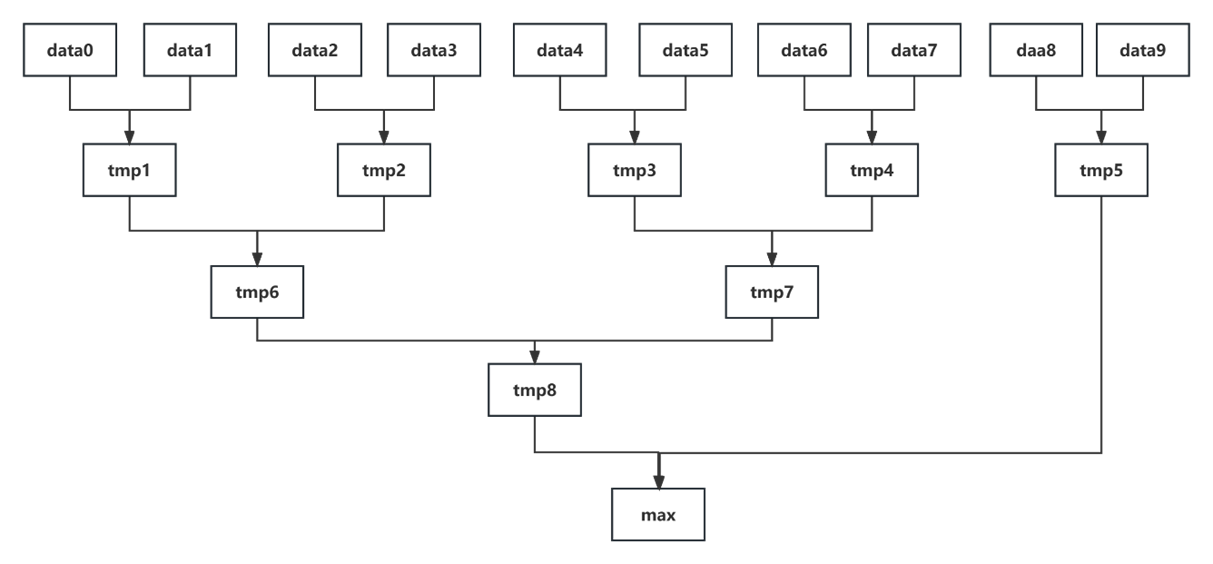
\includegraphics[width=0.8\linewidth]{Images/comptree.png}
        \caption{Sơ đồ khối cây so sánh 5 tầng}
        \label{fig:enter-label}
    \end{figure}

    \item Cơ chế pipeline:
    \begin{itemize}
        \item Stage 1 (Compute): Nhân-ma-trận và cộng bias từ ROM (1 chu kỳ)
        \item Stage 2 (Vote): So sánh 10 giá trị dense qua cây tournament (3 chu kỳ)
    \end{itemize}

    \item Triển khai phép toán signed MAC:
    \begin{verbatim}
        // Signed multiplication with sign extension
        mul_res[i] = {12'b0, data_in} * {{12{w[i][11]}}, w[i]}; 
        // Accumulation with 16-bit bias
        dense_temp[i] = dense[i] + mul_res[i][23:8];
    \end{verbatim}

    \item Tối ưu hóa phần cứng:
    \begin{itemize}
        \item Sử dụng DSP blocks cho phép nhân 12-bit thay vì LUT
        \item Shared weight loading qua SIPO110 tiết kiệm 78\% bus điều khiển
    \end{itemize}
\end{itemize}

\subsubsection{Thiết kế khối FullyConnect}
\begin{table}[H]
\centering
\caption{Module FullyConnect Signal Definitions}
\label{tab:fc_signals}
\begin{tabular}{llll}
\toprule
\textbf{Signal Name} & \textbf{Direction} & \textbf{Width} & \textbf{Description} \\
\midrule
clk & Input & 1 & System clock \\
rst & Input & 1 & Active-high reset \\
data\_in & Input & 12 & Input feature map (Q4.8) \\
w & Input & 120 & Weight value (Q4.8) \\
pos\_data & Output & 4 & Position counter \\
load\_weight & Output & 1 & Weight loading flag \\
cnn\_out & Output & 4 & Classification result \\
finish & Output & 1 & Operation completion flag \\
\bottomrule
\end{tabular}
\end{table}

\begin{itemize}
    \item Cơ chế hoạt động:
    \begin{itemize}
        \item Giai đoạn tính toán:
        \begin{itemize}
            \item Thực hiện phép nhân có dấu Q4.8 $\times$ Q4.8
            \item Cộng dồn với bias pre-load từ bộ nhớ ROM
            \item Pipeline 3 giai đoạn: Nhân $\rightarrow$ Cộng $\rightarrow$ So sánh
        \end{itemize}
        \item Giai đoạn voting:
        \begin{itemize}
            \item So sánh 10 giá trị dense theo cơ chế tournament sort
            \item Xuất kết quả lớp có giá trị lớn nhất (4-bit one-hot)
        \end{itemize}
    \end{itemize}
    
    \item Kiến trúc Pipeline:
    \begin{itemize}
        \item Stage 1: 10 bộ nhân song song (12-bit $\times$ 12-bit)
        \item Stage 2: 10 bộ cộng có dấu 16-bit với bias
        \item Stage 3: Cây so sánh 5 tầng để tìm max
    \end{itemize}
\end{itemize}

\subsubsection{Kiểm Thử \& Xác Minh}
\begin{table}[H]
\centering
\caption{FullyConnect Verification Plan}
\begin{tabular}{>{\bfseries}p{2.5cm}p{4cm}p{4cm}p{3cm}}
\toprule
\textbf{Test Category} & \textbf{Test Case} & \textbf{Verification Method} & \textbf{Expected Result} \\
\midrule
Reset Verification & Power-on reset & Assert reset, then release & All registers cleared, cnn\_out=15 \\
\hline
Weight Loading & Serial weight shifting & Input known weight pattern & Correct parallel output after 12 cycles \\
\hline
Basic Inference & All weights=1.0 & Input fixed value 1.0 & Correct dense[i] = bias[i] + 1.0 \\
\hline
Boundary Cases & Max Q4.8 input (7.996) & Input 12'h7FF with random weights & Proper saturated accumulation \\
\hline
Negative Values & Mixed sign weights & Alternate positive/negative weights & Correct signed arithmetic \\
\hline
Timing Control & Finish signal timing & Monitor pos\_data counter & finish=1 when pos\_data overflows \\
\hline
Comparison Logic & All dense equal & Set identical dense values & Any class selected (one-hot) \\
\hline
Bias Loading & ROM initialization & Check initial dense values & Match predefined biasrom.mem \\
\bottomrule
\end{tabular}
\end{table}

\begin{figure}[H]
    \centering
    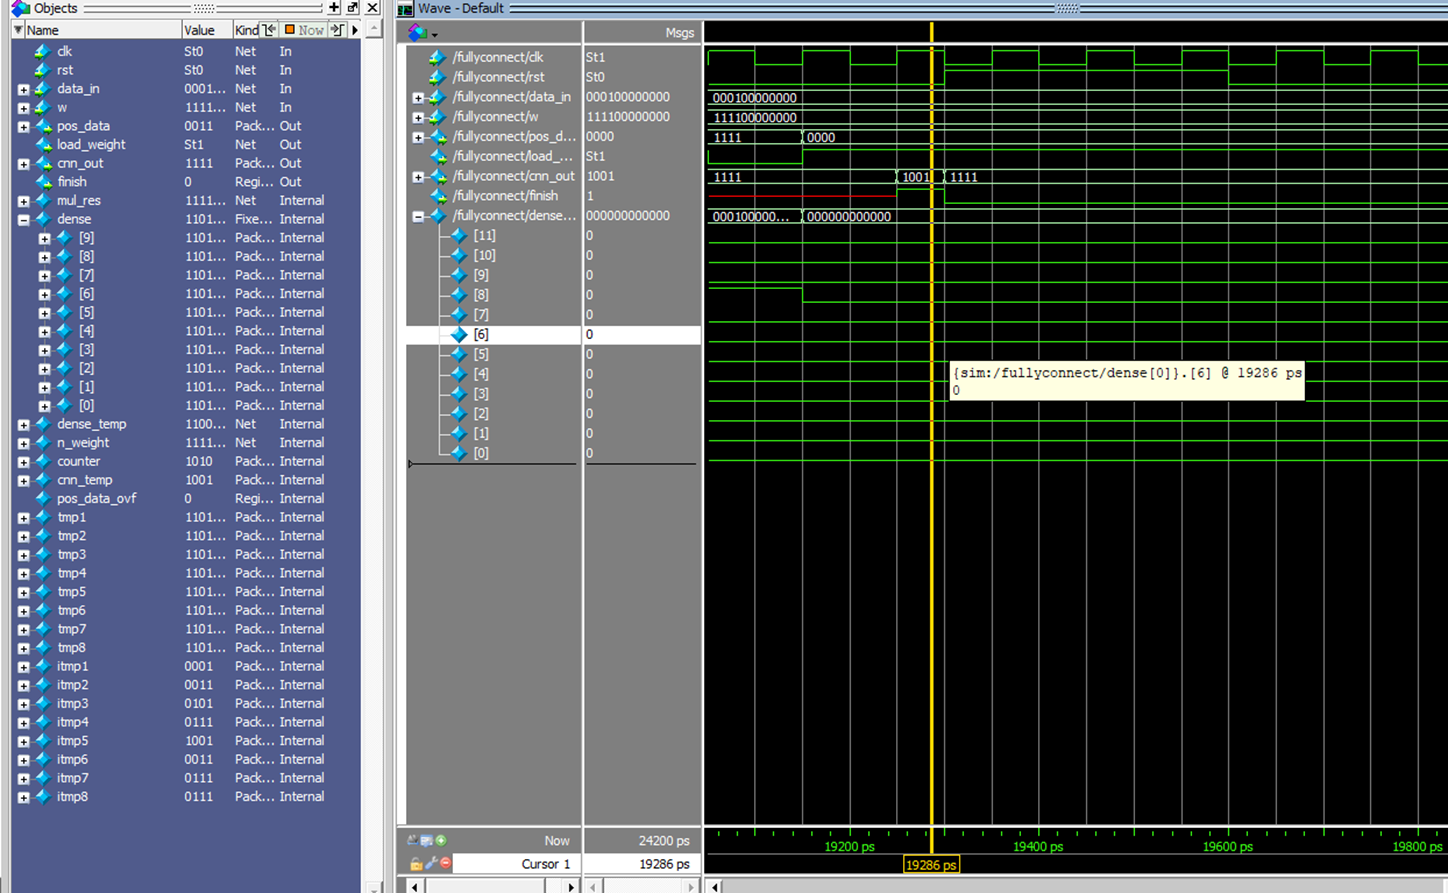
\includegraphics[width=0.9\linewidth]{Images/wavefc.png}
    \caption{Dạng sóng testbench với tất cả giá trị dense giống nhau}
    \label{fig:fc_wave}
\end{figure}
Với tất cả giá trị dense giống nhau khi đưa vào cây so sánh theo thuật toán cây so sánh nếu tất cả các giấ trị so sánh bằng nhau kết quả trả về sẽ là 9. \\
Viết code testbench và sử dụng chức năng monitor của Modelsim để kiểm tra các testcase
còn lại.

\begin{figure}[H]
    \centering
    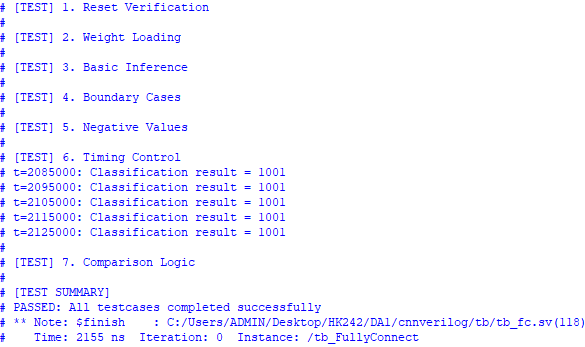
\includegraphics[width=0.75\linewidth]{Images/tbfc.png}
    \caption{Testbench Fully Connect}
    \label{fig:enter-label}
\end{figure}

\subsubsection{Synthesize}
Sử dụng phần mềm Gowin FPGA Designer để chạy synthesis ta có kết quả Netlist như hình \ref{fig:fc_synth}.
\begin{figure}[H]
    \centering
    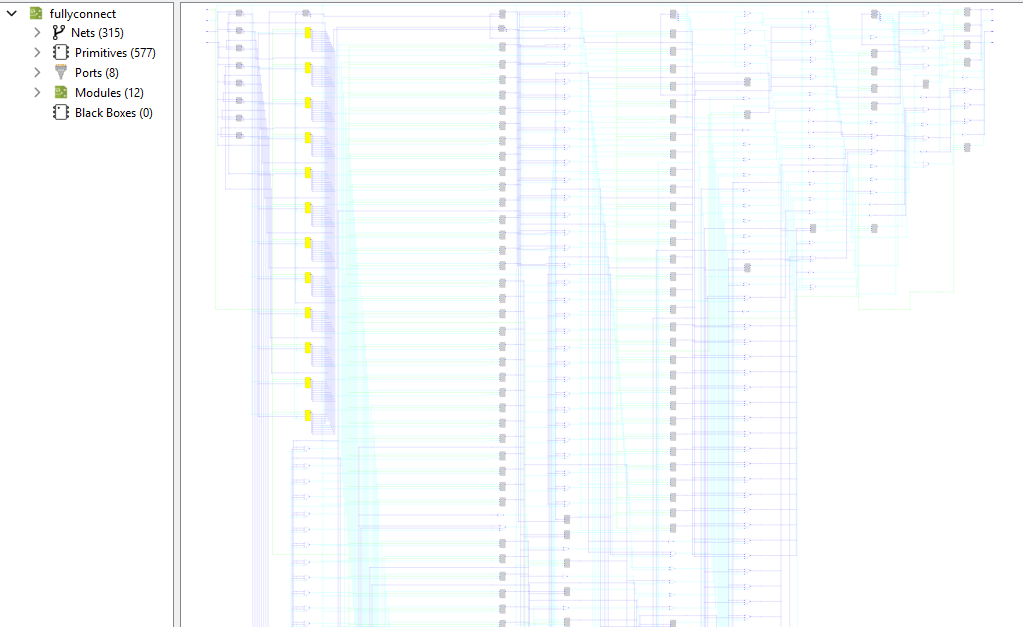
\includegraphics[width=0.75\linewidth]{Images/fcsynth.png}
    \caption{Kết quả netlist synthesis khối FullyConnect}
    \label{fig:fc_synth}
\end{figure}

Ta có được báo cáo tài nguyên sử dụng và timing như sau.

\begin{table}[h]
\centering
\caption{Báo cáo tài nguyên FPGA cho FullyConnect}
\label{tab:fc_resource}
\begin{tabular}{
    l
    S[table-format=3.0]
    @{\hspace{1em}}
    S[table-format=4.0]
    S[table-format=2.1]
}
\toprule
\multirow{2}{*}{\textbf{Tài nguyên}} & 
\multicolumn{2}{c}{\textbf{Sử dụng/Tổng}} & 
\multirow{2}{*}{\textbf{Utilization}} \\
& \multicolumn{2}{c}{(đơn vị)} & \\
\midrule
Logic & 550 & (310 LUT, 240 ALU) / 8640 & 7.0\% \\
\hline
Register & \multicolumn{2}{l}{182 / 6693} & 3.0\% \\
\quad $\bullet$ FF & \multicolumn{2}{l}{0 / 6693} & 0\% \\
\quad $\bullet$ Latch & \multicolumn{2}{l}{182 / 6693} & 3.0\% \\
\hline
DSP &  &  \\
\quad $\bullet$ MULT18X18 & 10 &  \\
\bottomrule
\end{tabular}
\end{table}

\begin{figure}[H]
    \centering
    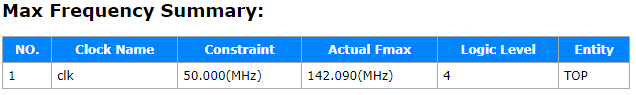
\includegraphics[width=0.9\linewidth]{Images/timingfc.png}
    \caption{Báo cáo timing khối Fully Connect}
    \label{fig:fc_timing}
\end{figure}

\subsection{Khối BSRam}

Ta sẽ phân vùng Ram như sau để lưu dữ liệu từng lớp.
\begin{table}[H]
\centering
\caption{Bảng memory map hệ thống CNN (14-bit địa chỉ, 12-bit dữ liệu)}
\label{tab:memory_map}
\begin{tabular}{|>{\ttfamily}c|>{\ttfamily}c|>{\ttfamily}c|l|}
\hline
\rowcolor{gray!20}
\textbf{Vùng} & \textbf{Địa chỉ bắt đầu} & \textbf{Kích thước} & \textbf{Mô tả} \\
\hline
% \rowcolor{convcolor}
PADDING & 14'd0 & 1 words & \multirow{2}{8cm}{Chứa zero dùng để làm padding cho CONV} \\
       & (0x0000) & (0x0001) & \\
\hline

\rowcolor{convcolor}
CONV1 & 14'd1 & 784 words & \multirow{2}{8cm}{Chứa dữ liệu 1 ảnh 28x28 đầu vào CONV1} \\
       & (0x0001) & (0x0310) & \\
\hline
\rowcolor{convcolor}
CONV2 & 14'd785 & 3136 words & \multirow{2}{8cm}{Chứa dữ liệu 4 ảnh 28x28 đầu vào CONV2} \\
       & (0x0311) & (0x0C40) & \\
\hline
\rowcolor{poolcolor}
MPOOL1 & 14'd3921 & 3136 words & Chứa dữ liệu 4 ảnh 28x28 đầu vào MPOOL1 \\
       & (0x0F51) & (0x0C40) & \\
\hline
\rowcolor{convcolor}
CONV3 & 14'd7057 & 784 words & Chứa dữ liệu 4 ảnh 14x14 đầu vào CONV3 \\
       & (0x1B91) & (0x0310) & \\
\hline
\rowcolor{convcolor}
CONV4 & 14'd7841 & 1568 words & Chứa dữ liệu 8 ảnh 14x14 đầu vào CONV4 \\
       & (0x1EA1) & (0x0620) & \\
\hline
\rowcolor{poolcolor}
MPOOL2 & 14'd9409 & 1568 words & Chứa dữ liệu 8 ảnh 14x14 đầu vào MPOOl2 \\
       & (0x24C1) & (0x0620) & \\
\hline
\rowcolor{convcolor}
CONV5 & 14'd10977 & 392 words & Chứa dữ liệu 8 ảnh 7x7 đầu vào CONV5 \\
       & (0x2AE1) & (0x0188) & \\
\hline
\rowcolor{poolcolor}
GMPOOL & 14'd11369 & 784 words & Chứa dữ liệu 16 ảnh 7x7 đầu vào GMPOOL \\
       & (0x2C69) & (0x0310) & \\
\hline
\rowcolor{densecolor}
DENSE & 14'd12153 & 16 words & Chứa dữ liệu 16 ảnh 1x1 đầu vào Fully Connect \\
       & (0x2F79) & (0x0010) & \\
\hline
TỔNG &  & 12169 words &  \\

\hline
\end{tabular}
\end{table}

Như vậy để có thể lưu trữ được tất cả dữ liệu cần thiết cho nhận diện số viết tay ta cần dùng bộ nhớ ram có kích thước khoảng 18kByte.
\begin{figure}[H]
    \centering
    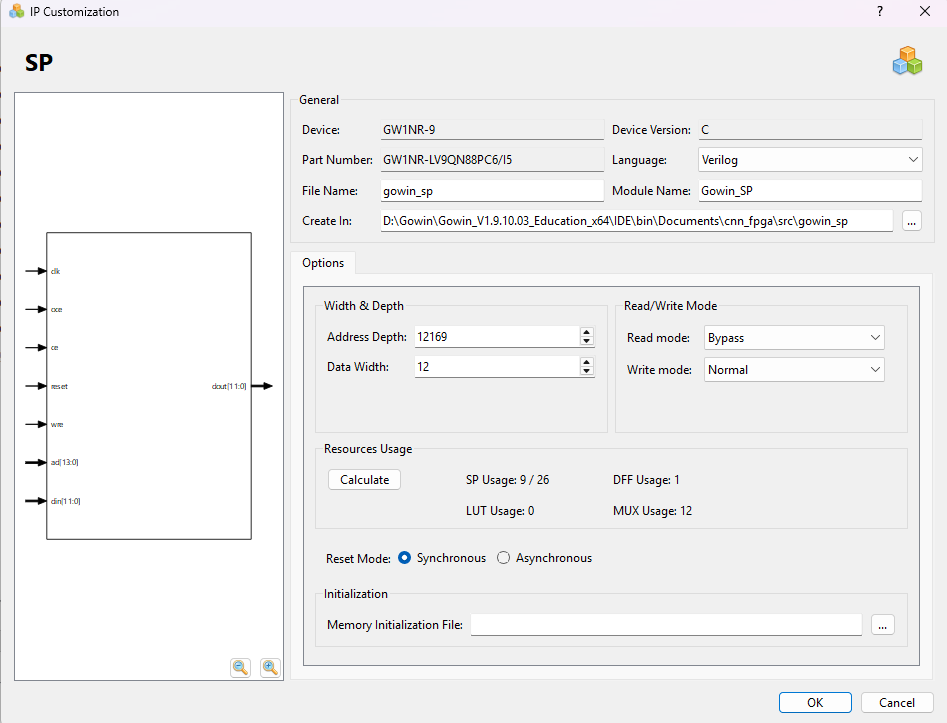
\includegraphics[width=0.75\linewidth]{Images/ipcoreram.png}
    \caption{BSRam ip core Gowin}
    \label{fig:enter-label}
\end{figure}
Để đơn giản việt thiết kế ta có thưeer dùng tính năng IP Core của tool Gowin để tạo khối BSRAM. Kit Tang Nano 9K hỗ trợ đến 26 khối BSRAM với kích thước mỗi khối là 16kBit. Theo hình ta thấy cần sử dụng 9 khối BSRAM tương ứng với 18kByte như tính toán bên trên.

\subsection{Các khối ROM chứa dữ liệu trọng số}
Triển khai mô hình AI trên phần cứng đòi hỏi chuyển đổi trọng số từ định dạng dấu phẩy động (float32) sang định dạng cố định (fixed-point) Q4.8 và nhị phân của lớp convolution. File .mem trong Verilog chứa dữ liệu nhị phân/hex, được sử dụng để khởi tạo bộ nhớ ROM/RAM.

\begin{figure}[H]
    \centering
    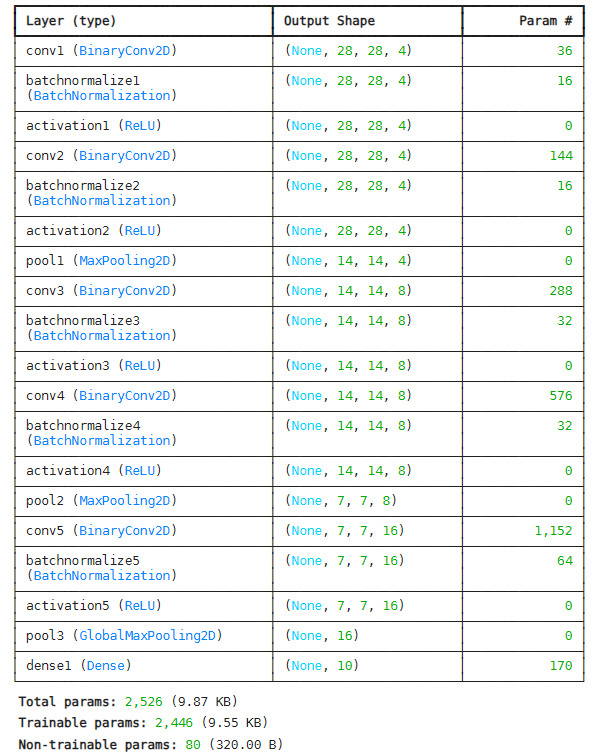
\includegraphics[width=0.75\linewidth]{Images/cnnmodel.png}
    \caption{Báo cáo trọng số từng lớp CNN}
    \label{fig:enter-label}
\end{figure}

\textbf{Các bước thực hiện}
\begin{itemize}
    \item B1: Trích xuất Trọng số từ CNN bằng cách sử dụng API của TensorFlow ( \texttt{model.layers[i].get\_weights()}).
    \item B2: Chuyển đổi sang Nhị phân
    \begin{itemize}
        \item Làm phẳng (flatten) filter 3x3 và chuyển đổi trọng số của lớp conv về dạng nhị phân ta được một chuối 9-bit tương ứng với 9 trọng số của filter 3x3.
        \item Tính toán trước hệ số $\theta$ và $\phi$ mà ta thiết kế theo 4 hệ số trọng số $\alpha,\beta,\gamma,\mu$ của lớp Batch Normalize và lượng tử vệ đinh dạng Q4.8.
        \item Lượng tử trọng số và bias của lớp fully connect về dạng Q4.8.
    \end{itemize}
    \item B3: Tạo File .mem cho Verilog
    \item B4: Khởi tạo bộ nhớ trong Verilog với từng khối ROM.
\end{itemize}
\textbf{Kích thước Rom}
\begin{itemize}
    \item Tổng các param của lớp conv là: $36+144+288+576+1152=2196$. Vậy ta cần 1 ROM chứa 244x9-bit để lưu trọng số lớp conv.
    \item Tổng các param của lớp batch normalize là: $16+16+32+32+64=160$ do ta đã giảm một nửa số param của lớp này nên còn 80 param. Vậy ta cần 1 ROM chứa 80x12-bit để lưu trọng số lớp Batch normalize.
    \item Tổng số param của lớp fully connect là 170 bỏ qua 10 trọng số bias được load sẵn ta cần 1 ROM chứa 160x12-bit để lưu trọng số lớp này.
\end{itemize}



\subsection{Khối điều khiển (FSM)}
\subsubsection{Tổng quan}
Dựa theo flow tính toán và sơ đồ của mạng CNN ta lập được một sơ đồ máy trạng thái như sau (Gộp 3 lớp BinaryConv + BatchNormalize + ReLU thành 1 trạng hái CONV):

\begin{figure}[H]
    \centering
    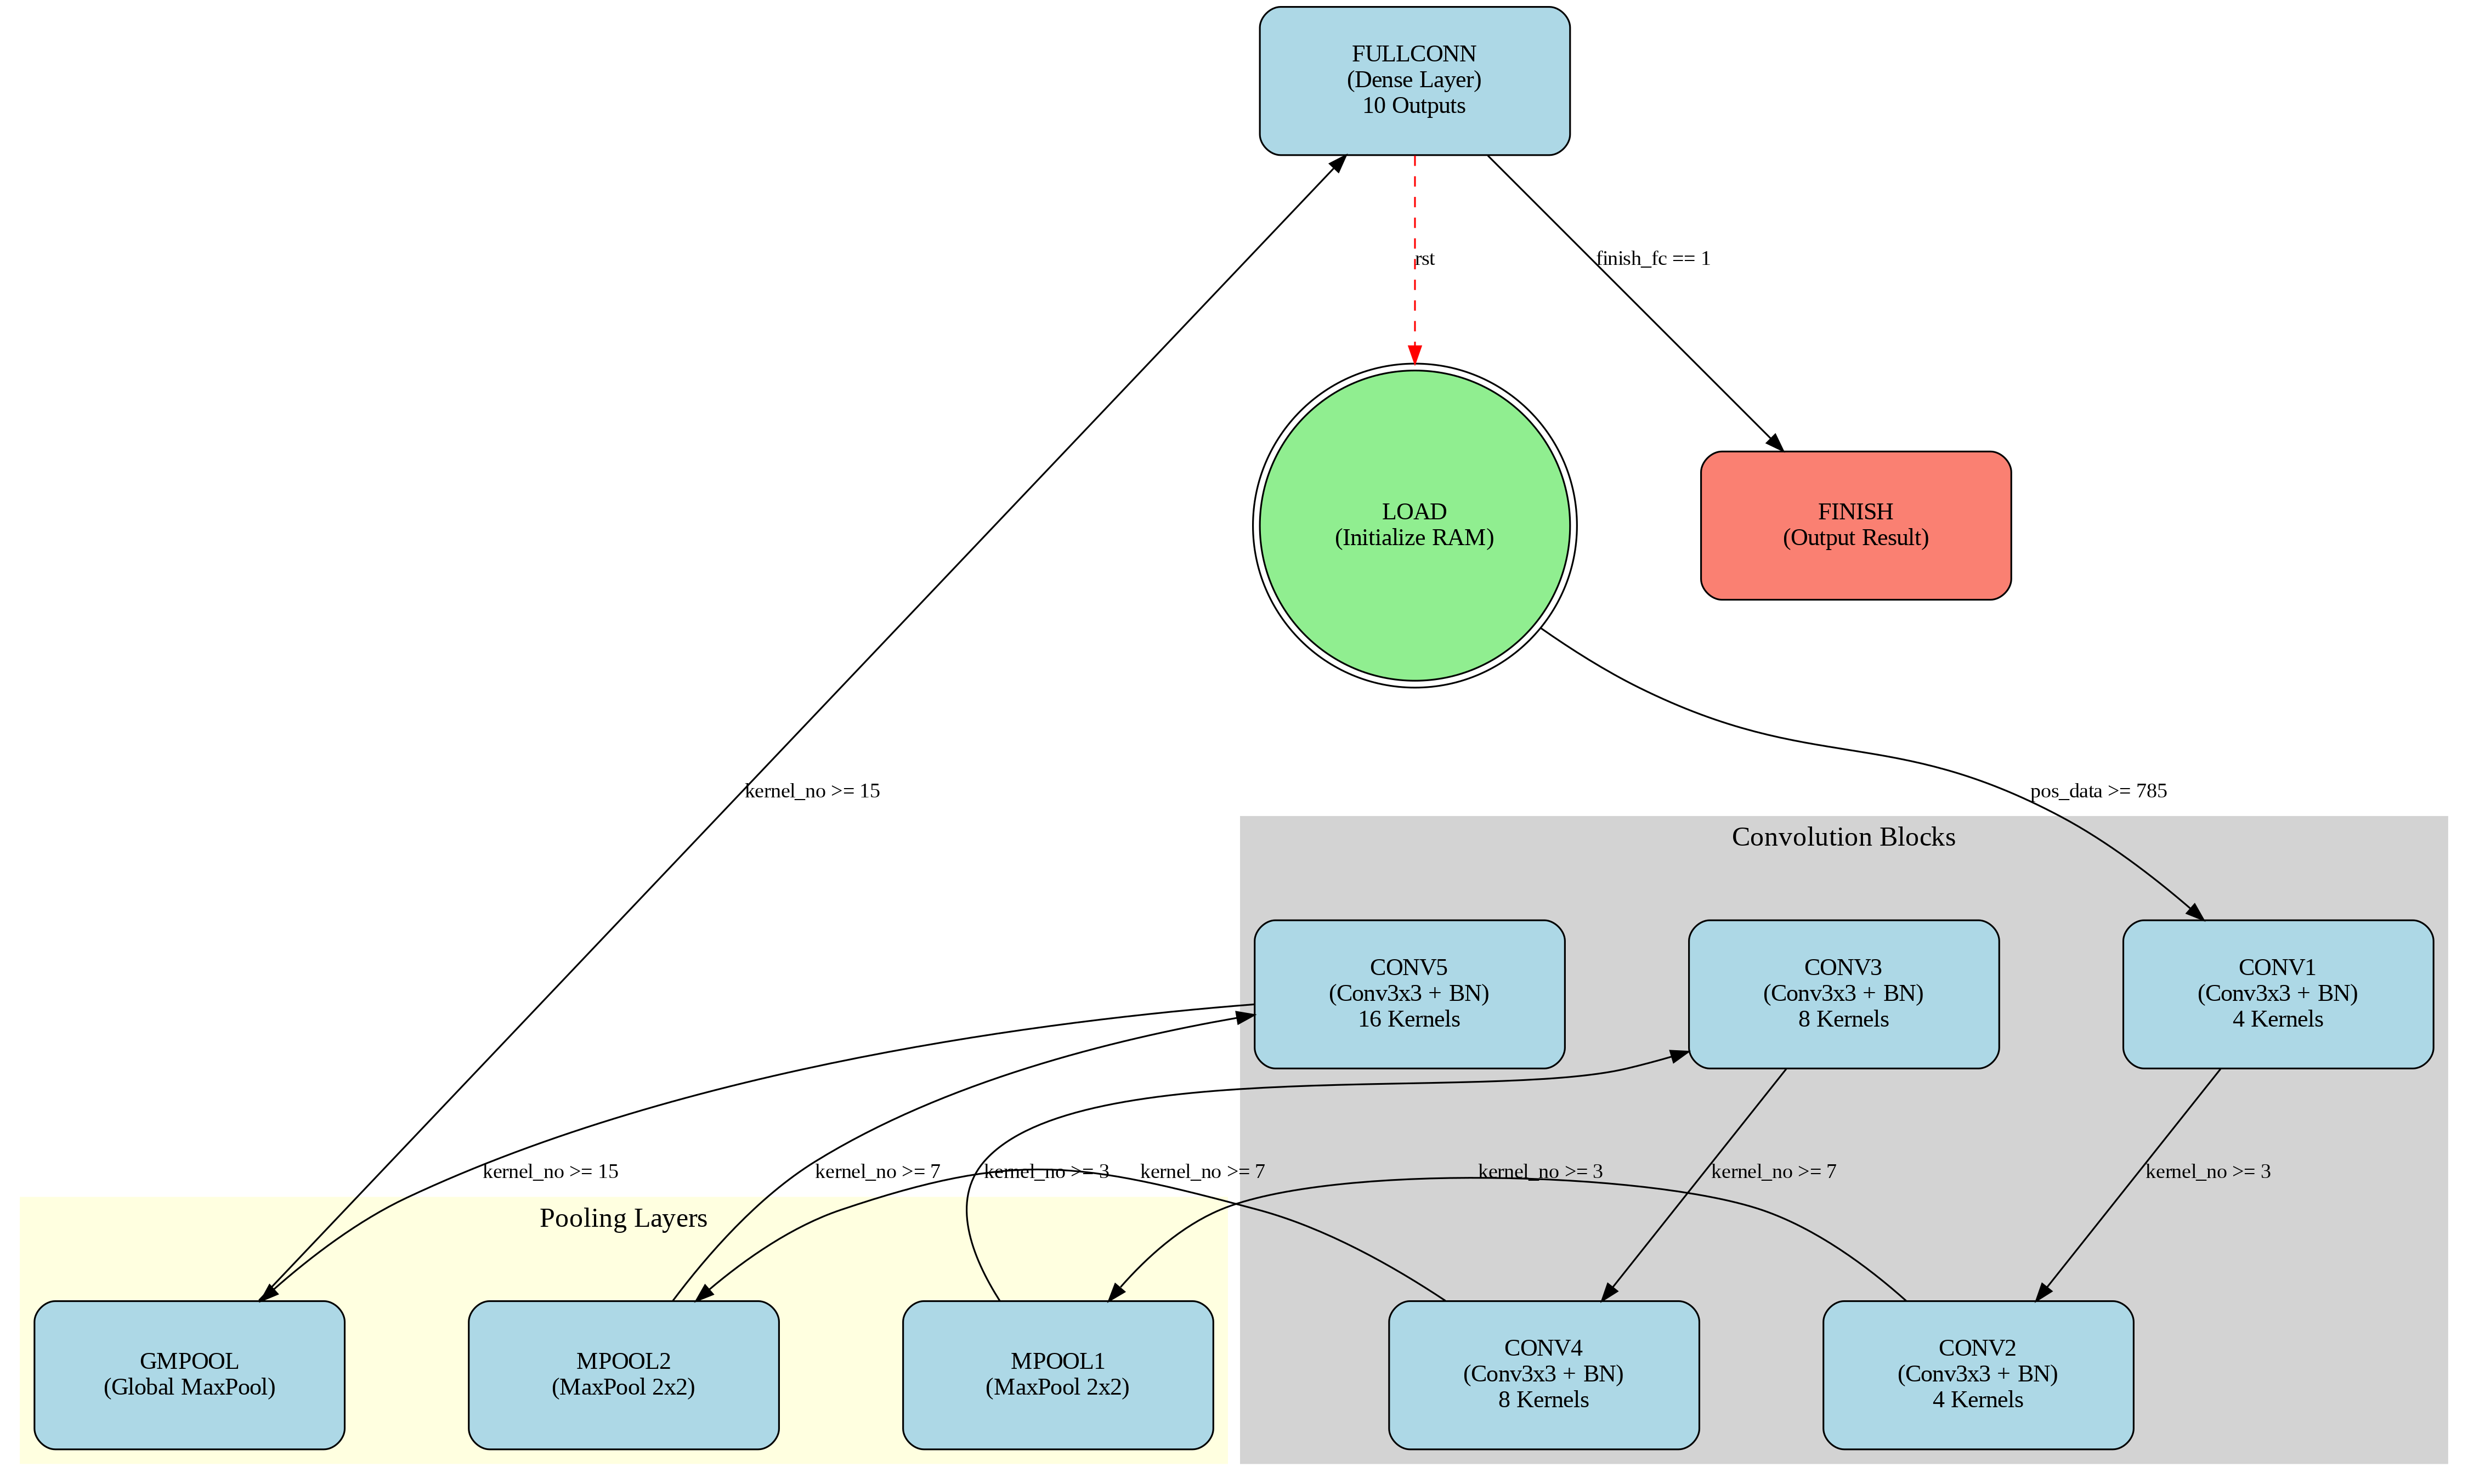
\includegraphics[width=0.9\linewidth]{Images/fsm.png}
    \caption{Sơ đồ trạng thái của khối điều khiển}
    \label{fig:enter-label}
\end{figure}
Ở các trạng thái khác nhau sẽ có tín hiệu điều khiển cho datapath khác nhau.

\subsubsection{Giai đoạn LOAD}
Ở giai đoạn này sẽ xuất các tín hiệu điều khiển để lưu ảnh mới 8-bit qua khối chuẩn hóa chuyển thành kiểu dữ liệu Q4.8 và lưu vào Bsram.
\begin{figure}[H]
    \centering
    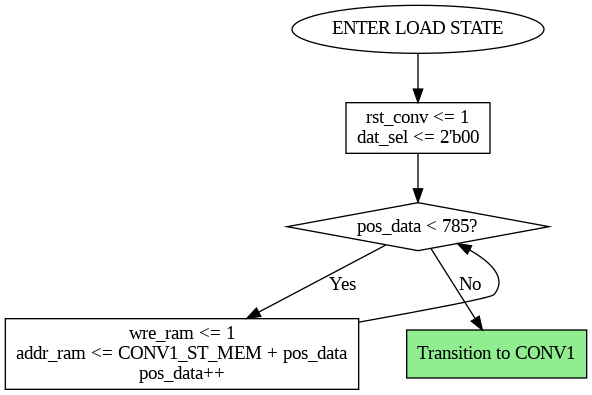
\includegraphics[width=0.75\linewidth]{Images/loadflow.png}
    \caption{Flow chart ở giai đoạn LOAD}
    \label{fig:enter-label}
\end{figure}

Kết thúc giai đoạn này ta sẽ có được 784 pixel dữ liệu hình ảnh đã được chuẩn hóa lưu ở trong Ram.

\subsubsection{Giai đoạn CONV1}
Ở giai đoạn ta cần điều khiển địa chỉ của ROM chứa trọng số của lớp Conv và BatchNormalize theo từng Kernel. Ngoài ra còn phải tính toán địa chỉ điểm ảnh của ảnh vừa được load vào trong Ram. Ảnh được load vào trong Ram là ảnh đã được làm phẳng do đó ta cần 2 thành ghi là \textit{x\_temp\_pos} và \textit{y\_temp\_pos} để thực hiện quá trình quét ảnh 2D của lớp Conv
\begin{figure}[H]
    \centering
    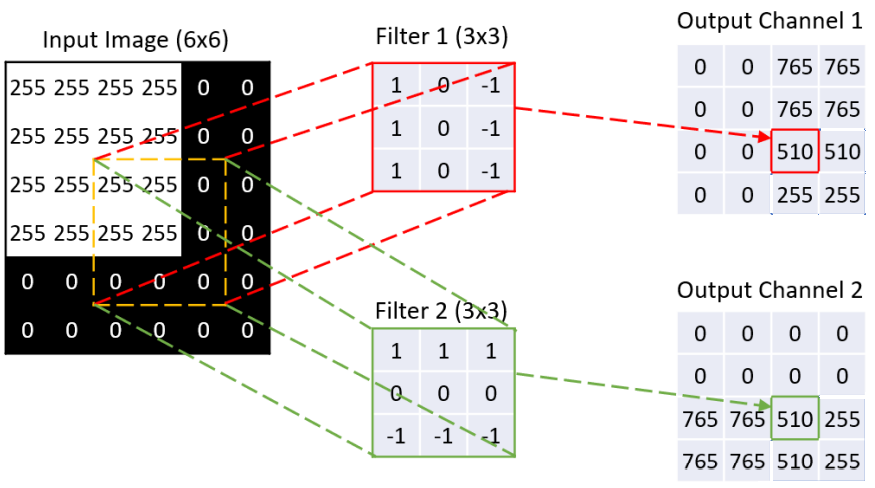
\includegraphics[width=0.75\linewidth]{Images/ohlc_filter.png}
    \caption{Quá trình quét ảnh 2D}
    \label{fig:filter}
\end{figure}
Ngoài 2 thanh ghi lưu tọa độ của điểm ảnh ta cần thêm 2 thanh ghi để lưu tọa độ 8 điểm ảnh lân cận. Vì như hình \ref{fig:filter} tất cả các Kernel (Filter) ta sử dụng trong mô hình này đều là 3x3 mỗi lần trượt của Filter sẽ lấy 9 giá trị điểm ảnh nhân tích chập với trọng số để tạo ra được điểm ảnh mới ở ngõ ra. \\
Và theo như mô hình ta chọn lúc đầu kích thước ảnh sau khi qua lớp Conv sẽ giữ nguyên (VD: 28x28) nhưng vì Kernel có size là 3x3 theo thực tế kích thước ảnh ngõ ra sẽ giảm 2 pixel (VD: 26x26). Vì thế ta sử dụng kỹ thuật Padding là các viền ngoài của ảnh ngõ vào sẽ cho bằng 0. Và theo như giải thuật trên ta sẽ thiết kế sao cho dựa vào 4 giá trị tọa độ điểm ảnh để phát hiện ra trường hợp điểm ảnh Padding.
\begin{figure}[H]
    \centering
    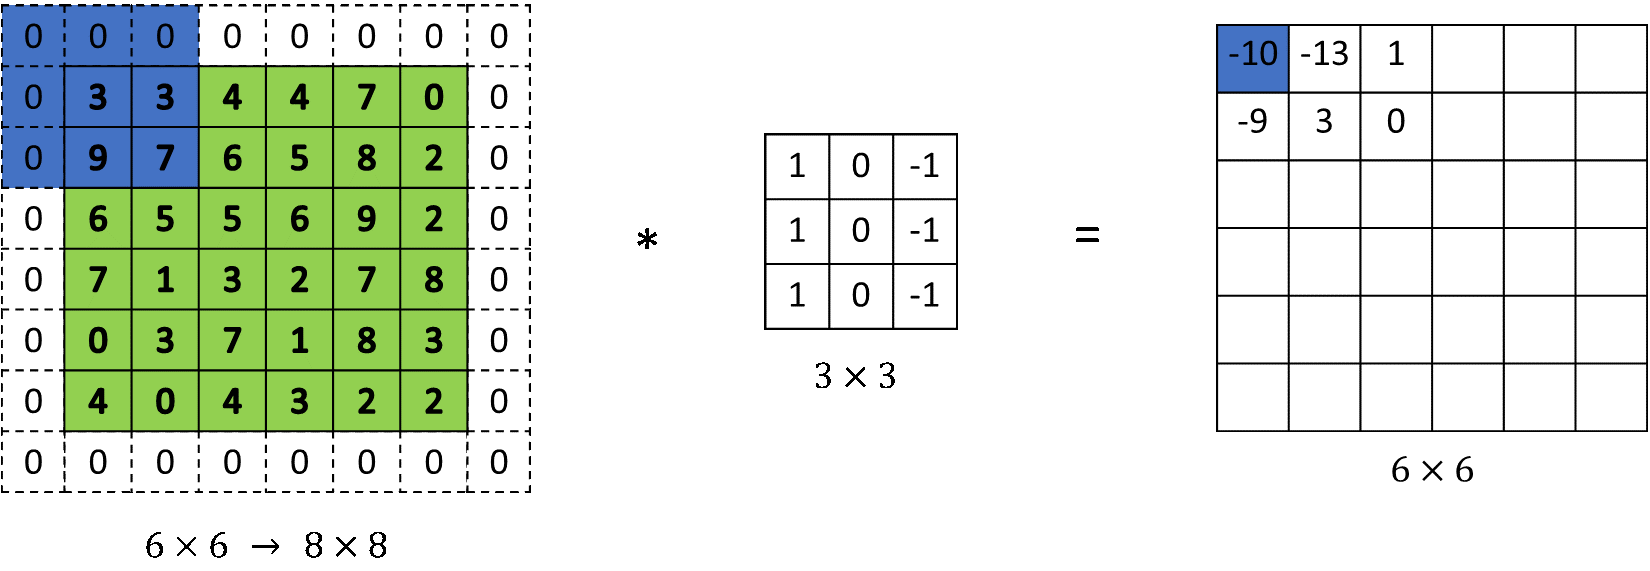
\includegraphics[width=0.9\linewidth]{Images/R.png}
    \caption{Padding cho lớp convolution}
    \label{fig:enter-label}
\end{figure}

Từ các ý trên ta có được các tín hiệu điều khiển như sau:


\begin{figure}[H]
    \centering
    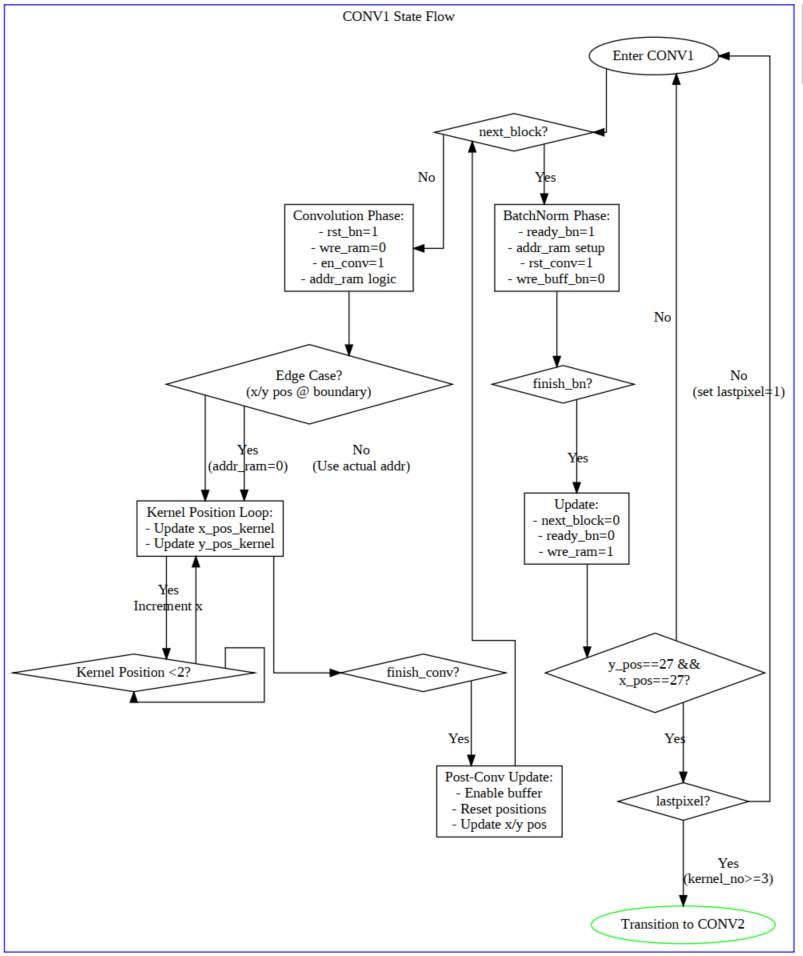
\includegraphics[width=0.75\linewidth]{Images/conv1flow.png}
    \caption{Flowchart CONV1}
    \label{fig:enter-label}
\end{figure}

Kết thúc giai đoạn CONV1 ta sẽ có được 4 kênh ảnh 28x28 mới lưu ở trong Ram và tiếp tục đến giai đoạn CONV2

\subsubsection{Giai đoạn CONV2}
Ở giai đoạn CONV2 sẽ tương tự giai đoạn đầu tiên, tuy nhiên số lượng ảnh kênh ngõ vào đã tăng lên thành 4 kênh. Như vậy ở mỗi Kernel ứng với mỗi kênh ảnh sẽ có mỗi Filter khác nhau (Window). 
\begin{figure}[H]
    \centering
    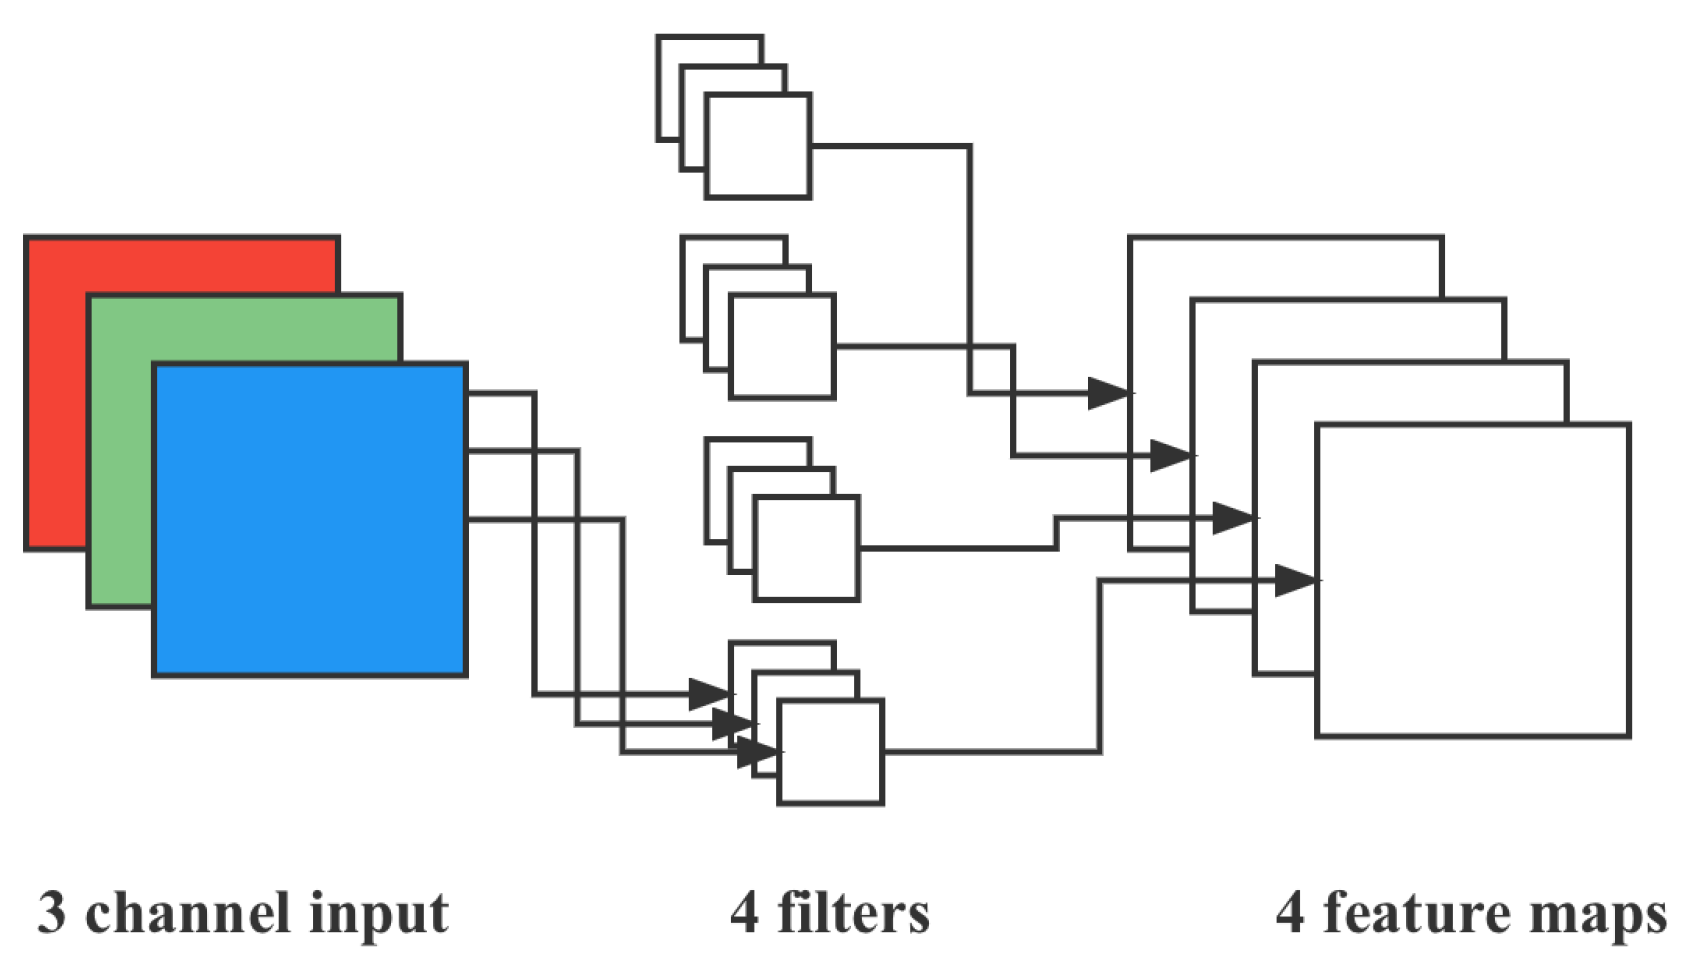
\includegraphics[width=0.75\linewidth]{Images/drones-06-00152-g010.png}
    \caption{Tích chập với ngõ vào nhiều kênh}
    \label{fig:enter-label}
\end{figure}
Vì thế tại mỗi điểm ảnh của mỗi kênh ngõ ra CONV2 sẽ là tổng tích chập của 4 kênh ảnh ngõ vào và 4 Window nên trong sơ đồ thiết kế phần cứng ta mới có thêm thanh ghi đệm Bnorm Reg trước khối BatchNormalize và bộ cộng để thực hiện điều này. Lúc này ở giai đoạn CONV2 ta cần phối hợp điều khiển thêm 2 tín hiệu là \textit{rst\_buff\_bn} và \textit{wre\_buff\_bn} để reset và cho phép ghi thanh ghi đệm này.
\begin{figure}[H]
    \centering
    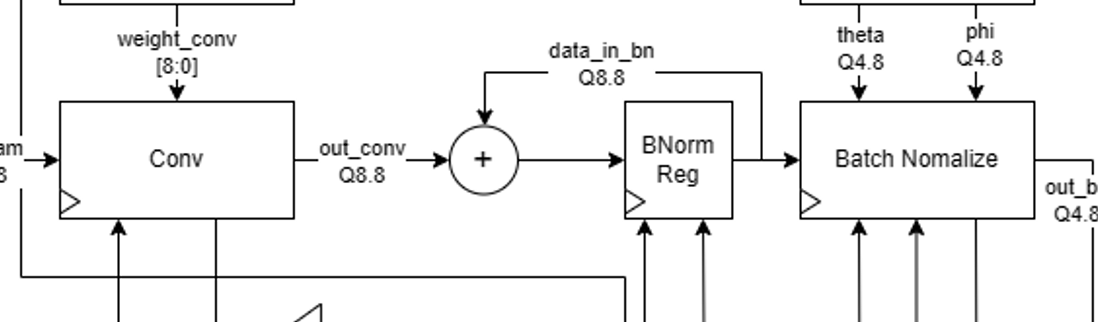
\includegraphics[width=0.75\linewidth]{Images/buffbn.png}
    \caption{Thanh ghi đệm Bnorm}
    \label{fig:enter-label}
\end{figure}
Ta lập được sơ đồ điều khiển các tín hiệu như sau:

\begin{figure}[H]
    \centering
    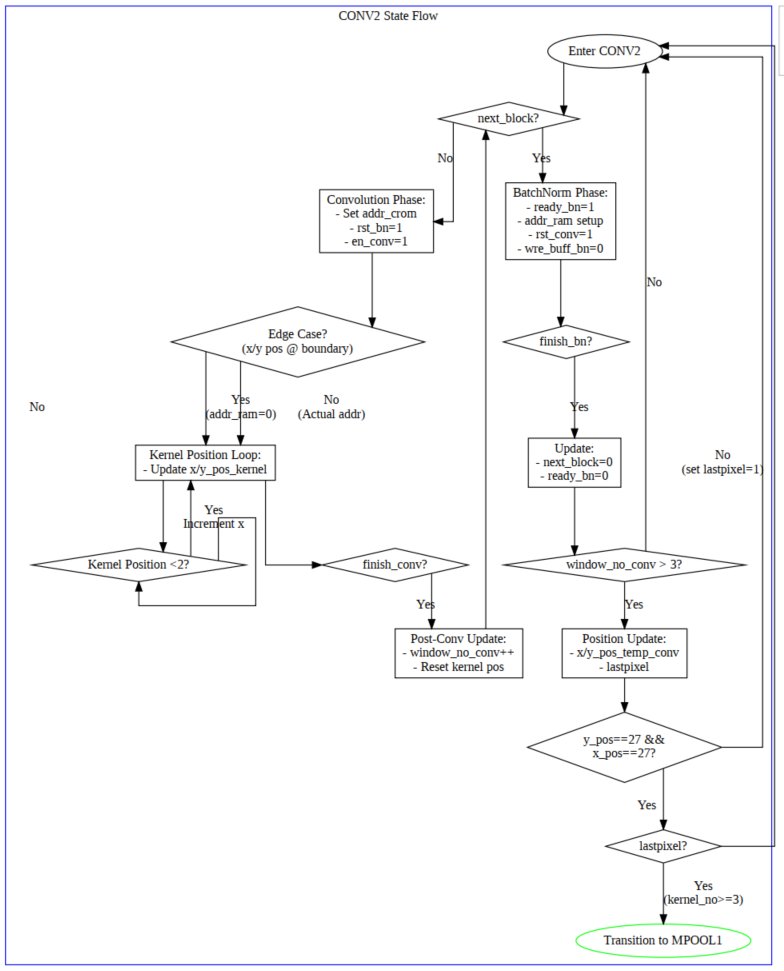
\includegraphics[width=0.75\linewidth]{Images/conv2flow.png}
    \caption{Flowchart CONV2}
    \label{fig:enter-label}
\end{figure}

Kết thúc giai đoạn CONV2 ta sẽ có được 4 kênh ảnh 28x28 mới và tiếp tục đến giai đoạn MAXPOOL1

\subsubsection{Giai đoạn MAXPOOL1}
Với giai đoạn max pooling 2D này ta sẽ so sánh 4 giá trị điểm ảnh trong vùng không gian 2x2 trên ảnh 2 chiều và chọn ra điểm ảnh có giá trị lớn nhất. Với kỹ thuật này sẽ giảm nửa chiều dữ liệu ngõ vào cho lớp sau.

\begin{figure}[H]
    \centering
    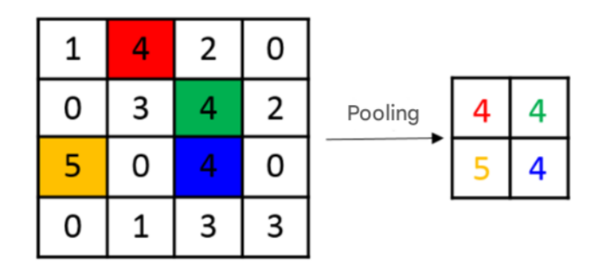
\includegraphics[width=0.75\linewidth]{Images/pooling.png}
    \caption{Maxpooling 2D}
    \label{fig:enter-label}
\end{figure}

Ta lập được sơ đồ điều khiển các tín hiệu cho giai đoạn max pooling như sau:

\begin{figure}[H]
    \centering
    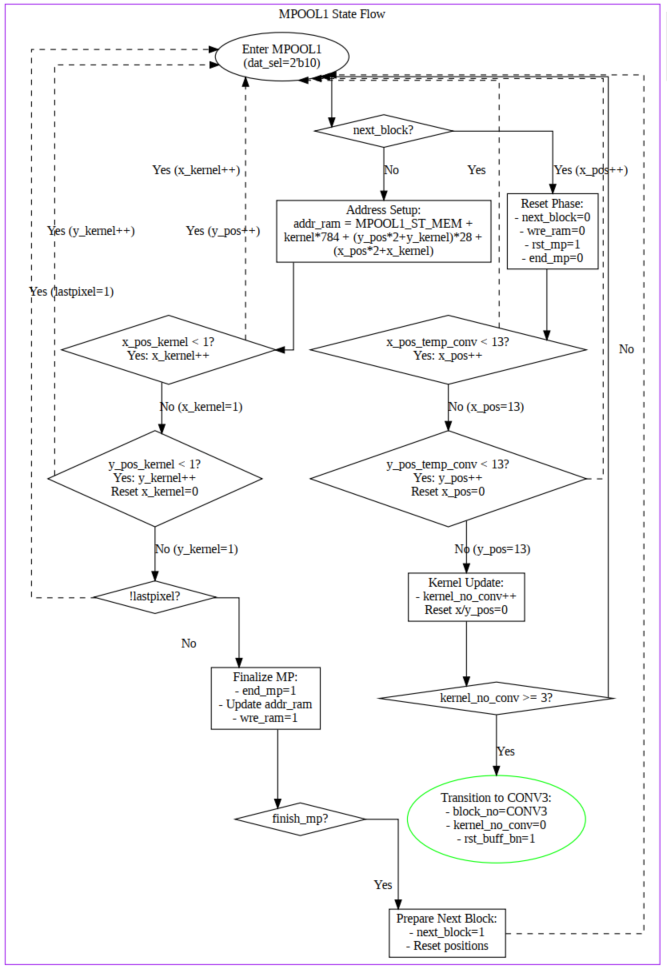
\includegraphics[width=0.75\linewidth]{Images/mpoolflow.png}
    \caption{Flowchart MAXPOOL1}
    \label{fig:enter-label}
\end{figure}
Kết thúc giai đoạn MAXPOOL1 ta sẽ có được 4 kênh ảnh 14x14 mới lưu ở trong Ram và tiếp tục đến giai đoạn CONV3

\subsubsection{Giai đoạn CONV3}
Giai đoạn này gần giống với CONV2 với số Kernel là 8 và số Window là 4. Và dữ liệu hình ảnh lúc này là 14x14 nên ta cần giảm số vòng lặp và thông số vị trí vùng Padding.\\
Kết thúc giai đoạn CONV3 ta sẽ có được 8 kênh ảnh 14x14 mới lưu ở trong Ram và tiếp tục đến giai đoạn CONV4.

\subsubsection{Giai đoạn CONV4}
Giai đoạn này giống với giai đoạn CONV3 với số lượng Window lúc này là 8.\\
Kết thúc giai đoạn CONV4 ta sẽ có được 8 kênh ảnh 14x14 mới lưu ở trong Ram và tiếp tục đến giai đoạn MAXPOOL2.

\subsubsection{Giai đoạn MAXPOOL2}
Tương tự giai đoạn MAXPOOL1 lúc này ta sẽ giảm một nửa dữ liệu. Lúc này dữ liệu ảnh cho giai CONV5 sau là 8 kênh anh 7x7.

\subsubsection{Giai đoạn CONV5}
Giai đoạn này giống với các giai đoạn CONV trên với số lượng Kernel là 16, Window là 8 tương ứng với 8 kênh ảnh 7x7 ở ngõ vào.\\
Kết thúc giai đoạn CONV5 ta sẽ có được 16 kênh ảnh 7x7 mới lưu ở trong Ram và tiếp tục đến giai đoạn GMPOOL.

\subsubsection{Giai đoạn GMPOOL}
Như đã nói ở các phần trước nhằm để giảm số lượng trọng số và tính toán ở lớp Fully Connect ta sử dụng kỹ thuật giảm chiều dữ liệu này với 16 kênh ảnh 7x7 từ giai đoạn trước đó.
\begin{figure}[H]
    \centering
    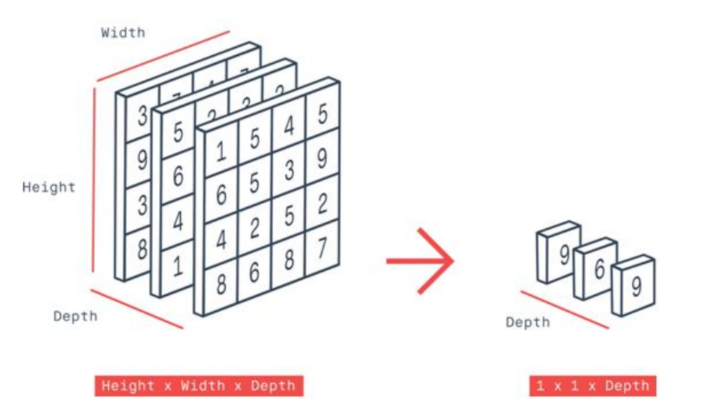
\includegraphics[width=0.75\linewidth]{Images/gmpool2.png}
    \caption{Kỹ thuật global max pool}
    \label{fig:enter-label}
\end{figure}
Điều khiển các tín hiệu tướng tự Max Pooling ta có được flow chart sau:
\begin{figure}[H]
    \centering
    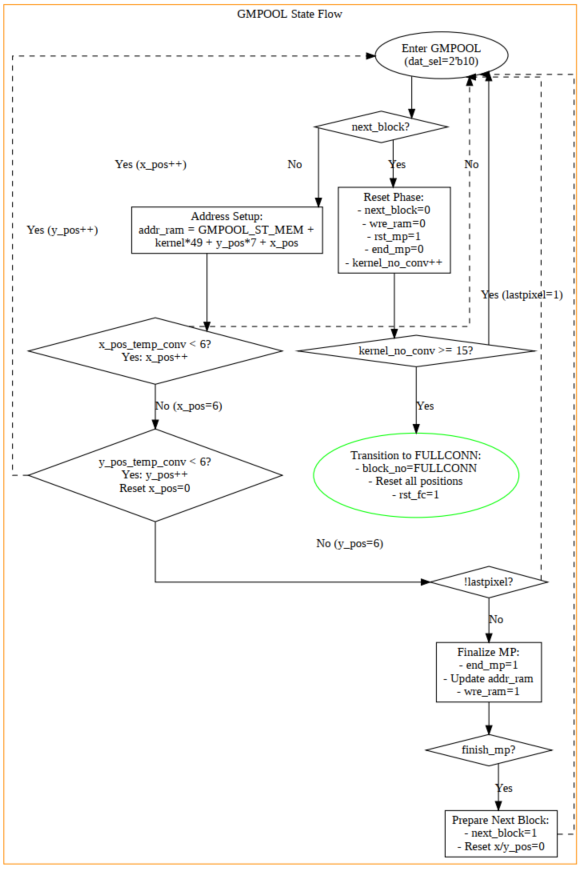
\includegraphics[width=0.75\linewidth]{Images/gmpoolflow.png}
    \caption{Flowchart GlobalMaxPooL}
    \label{fig:enter-label}
\end{figure}
Kết thúc giai đoạn GMPOOL ta sẽ có được 16 kênh ảnh 1x1 mới lưu ở trong Ram và tiếp tục đến giai đoạn FULLYCONN.

\subsubsection{Giai đoạn FULLYCONN}
Với ngõ vào là 16 kênh tương ứng ta có 16 Window, ngõ ra 10 kênh ứng với 10 Kernel. Sử dụng các thanh ghi để làm bộ đếm để lấy đúng dữ liệu trọng số ứng với Kernel và Window từ ROM và đưa váo khối FullyConnect.

\begin{figure}[H]
    \centering
    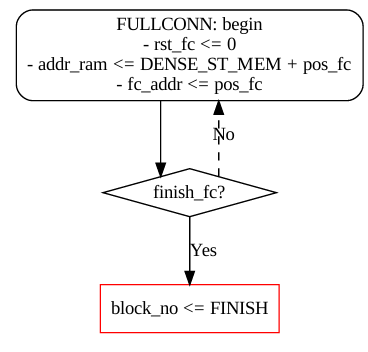
\includegraphics[width=0.5\linewidth]{Images/fcflow.png}
    \caption{Flowchart FULLYCONN}
    \label{fig:enter-label}
\end{figure}

Kết thúc quá trình load dữ liệu khối fully connect sẽ tự tính toàn và so sánh để đưa ra kết quả dự đoán số viết tay. Máy trạng thái sẽ chuyển qua trạng thái FINISH, kich hoạt cờ finish, để thực hiện chu trình dự đoán tiếp theo chỉ cần đưa tín hiệu reset cho máy trạng thái. 

\subsection{CNN Top}
\subsubsection{Thiết kế khối CNN Top}
Dựa vào sơ đồ thiết kế phần cứng (Hình \ref{fig:tkpc}) ta kết nối khối điều khiển và datapath với nhau để hoàn chỉnh module nhận diện số viết tay.
\begin{table}[H]
\centering
\caption{CNN Module Signal Definitions}
\label{tab:cnn_signals}
\begin{tabular}{llll}
\toprule
\textbf{Signal Name} & \textbf{Direction} & \textbf{Width} & \textbf{Description} \\ 
\midrule
clk & Input & 1 & System clock \\
rst & Input & 1 & Active-high reset \\
en & Input & 1 & Module enable control \\
data\_in & Input & 8 & Input pixel data (unsigned byte) \\ 
pos\_data & Output & 10 & Position counter/address bus \\
finish & Output & 1 & Operation completion flag \\
cnn\_out & Output & 4 & Classification result (0-9) \\ 
\bottomrule
\end{tabular}
\end{table}

\subsubsection{Synthesize}
Sử dụng tool Gowin để synthesis ta có báo cáo sử dụng tài nguyên như bảng \ref{tab:resource_usage_summary}.
\begin{table}[H]
\centering
\caption{Resource Usage Summary}
\label{tab:resource_usage_summary}
\begin{tabular}{ll}
\toprule
\textbf{Resource} & \textbf{Usage} \\
\midrule
I/O Port & 26 \\
I/O Buf & 25 \\
\quad $\bullet$ IBUF & 10 \\
\quad $\bullet$ OBUF & 15 \\
Register & 410 \\
\quad $\bullet$ DFF & 16 \\
\quad $\bullet$ DFFE & 34 \\
\quad $\bullet$ DFFRE & 1 \\
\quad $\bullet$ DFFPE & 103 \\
\quad $\bullet$ DFFC & 6 \\
\quad $\bullet$ DFFCE & 250 \\
LUT & 1353 \\
\quad $\bullet$ LUT2 & 289 \\
\quad $\bullet$ LUT3 & 352 \\
\quad $\bullet$ LUT4 & 712 \\
ALU & 1039 \\
\quad $\bullet$ ALU & 1039 \\
SSRAM & 3 \\
\quad $\bullet$ RAM16S4 & 3 \\
INV & 17 \\
\quad $\bullet$ INV & 17 \\
DSP & - \\
\quad $\bullet$ MULT18X18 & 10 \\
\quad $\bullet$ MULTADDALU18X18 & 5 \\
BSRAM & 15 \\
\quad $\bullet$ SP & 12 \\
\quad $\bullet$ pROM & 2 \\
\quad $\bullet$ pROMX9 & 1 \\
\bottomrule
\end{tabular}
\end{table}

Ta thấy thiết kế sử dụng rất ít tài nguyên với 2427 LUT, 410 thanh ghi flipflop và 15x16kbit bộ nhớ Ram.
\begin{table}[H]
\centering
\caption{Resource Utilization Summary}
\label{tab:resource_utilization_summary}
\begin{tabular}{l r@{\hspace{1em}}l S[table-format=2.1]}
\toprule
\multirow{2}{*}{\textbf{Resource}} & 
\multicolumn{2}{c}{\textbf{Used/Total}} & 
\multirow{2}{*}{\textbf{Utilization}} \\
& \multicolumn{2}{c}{(units)} & \\
\midrule
Logic & 2427 (1370 LUT, 1039 ALU, 3 RAM16) & / 8640 & 29.0\% \\
Register & 410 & / 6693 & 7.0\% \\
\quad $\bullet$ Register as Latch & 0 & / 6693 & 0.0\% \\
\quad $\bullet$ Register as FF & 410 & / 6693 & 7.0\% \\
BSRAM & 15 & / 26 & 58.0\% \\
\bottomrule
\end{tabular}
\end{table}

\subsubsection{Verification Plan}
\begin{table}[H]
\centering
\caption{CNN Module Verification Plan}
\begin{tabular}{>{\bfseries}p{2.5cm}p{4cm}p{4cm}p{3cm}}
\toprule
\textbf{Test Category} & \textbf{Test Case} & \textbf{Verification Method} & \textbf{Expected Result} \\
\midrule

Reset Verification & Power-on reset & Assert reset for 10 cycles & All states reset to LOAD, pos\_data=0, finish=0 \\
\hline
Convolution Layers & CONV1 edge pixels & Input boundary coordinates (x=0, y=0) & Zero-padded address (addr\_ram=0) selected \\
\hline
BatchNorm Integration & Post-CONV1 processing & Monitor bn\_addr and wre\_buff\_bn & Correct BN parameters applied to conv output \\
\hline
Max Pooling & MPOOL1 downsampling & Input 4x4 pattern with max=255 & Output 2x2 max values at correct addresses \\
\hline
State Transitions & CONV1→CONV2 transition & Trigger finish\_bn signal & block\_no increments to CONV2 within 1 cycle \\
\hline
Memory Addressing & CONV3 weight fetching & Check addr\_crom during computation & Correct CROM offset (20 + kernel\_no*4 + window\_no) \\
\hline
Global Pooling & GMPOOL operation & Feed 7x7 input with single peak & Maximum value stored at DENSE\_ST\_MEM \\
\hline
Full Connection & Final classification & Load precomputed GMPOOL outputs & cnn\_out matches MNIST label (one-hot) \\
\hline
Error Recovery & Mid-process reset & Assert rst during CONV2 operation & Immediate return to LOAD state \\
\hline
MNIST Accuracy & 10k test images & Compare cnn\_out with labels & ≥98\% classification accuracy \\

\bottomrule
\end{tabular}
\end{table}
Từ kế hoạch kiểm thử trên ta sẽ kiểm tra thiết kế ở phần sau.
\newpage
\section{KIỂM TRA THIẾT KẾ}

\subsection{Simulation}
Dựa vào kế hoạch kiểm thử ta tạo một testbench gồm thanh ghi lưu 10000 dữ liệu ảnh từ Test-set MNIST đã được làm phẳng và chuyển thành dạng nhị phân 8-bit và thanh ghi chứa label của từng ảnh. Tạo vòng lặp để lần lượt đưa từng pixel ảnh vào khối DUT để nhận diện đưa qua bộ Checker để so sánh kết quả với label của ảnh và đưa ra console. 
\begin{figure}[H]
    \centering
    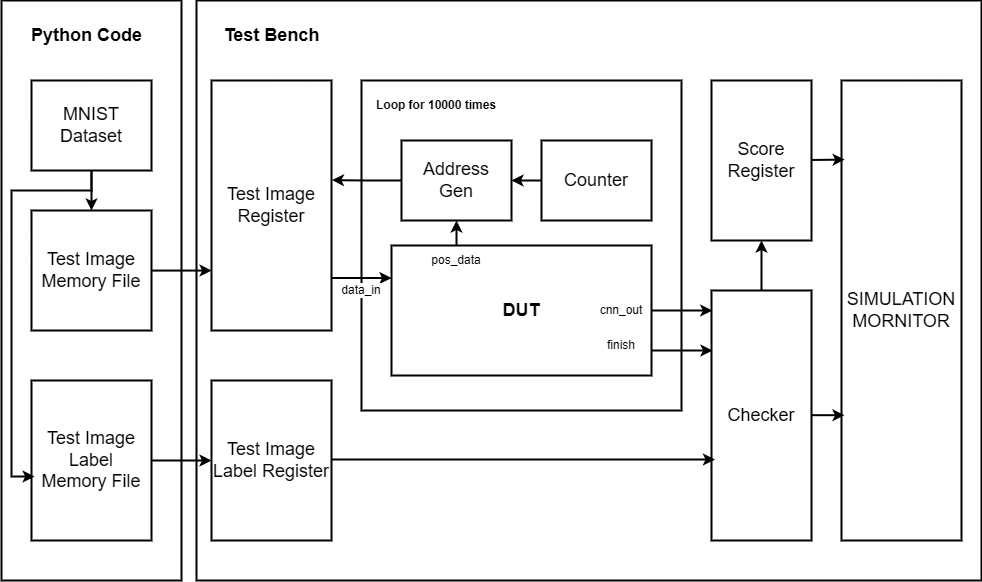
\includegraphics[width=1\linewidth]{Images/cnn_dut_mnist_test.drawio.png}
    \caption{Sơ đồ khối test simulation}
    \label{fig:enter-label}
\end{figure}

Dưới đây là các hình so sánh ngõ ra từng lớp khi chạy tính toán CNN trên FPGA ta thiết kế và model CNN chạy trên Tensorflow. Dữ liệu ảnh từng lớp ngõ ra ta lấy bằng cách dùng tính năng \textit{Export data patterns} để lấy dữ liệu lưu trong khối BSRam và dựa vào bảng memory map \ref{tab:memory_map} để lấy ra ảnh của từng lớp.
\begin{figure}[H]
\centering
    \begin{subfigure}[b]{0.45\linewidth}
        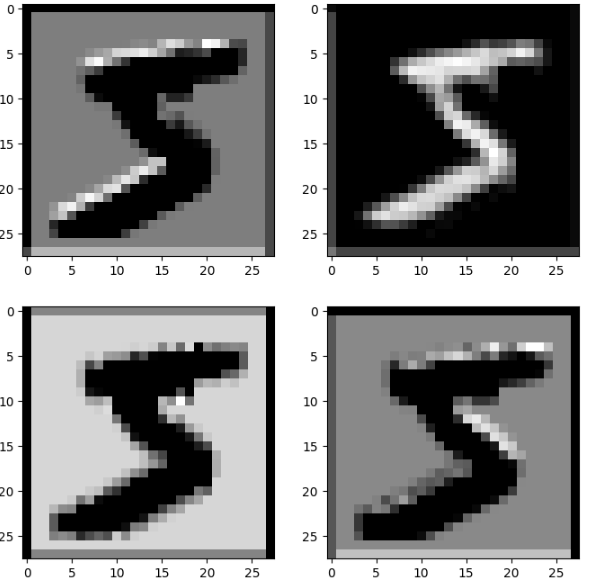
\includegraphics[width=\linewidth]{Images/fpgac1.png}
        \caption{FPGA}
        \label{fig:enter-label}
    \end{subfigure}
    \begin{subfigure}[b]{0.45\linewidth}
        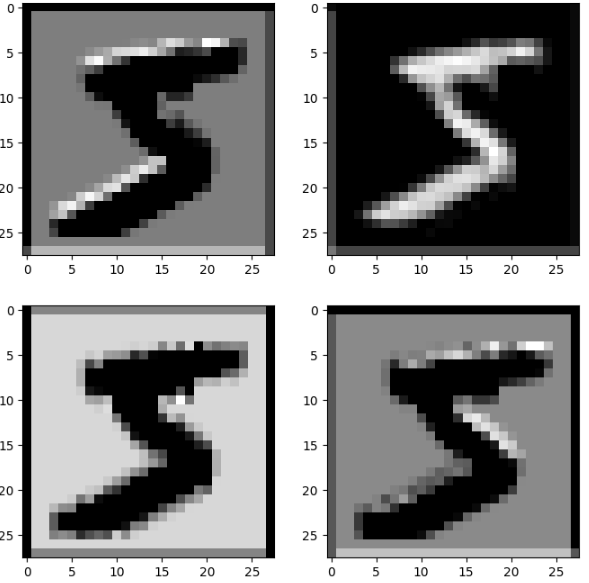
\includegraphics[width=\linewidth]{Images/cnnc1.png}
        \caption{Tensorflow}
        \label{fig:enter-label}
    \end{subfigure}
    \caption{Ảnh ngõ ra lớp Conv1}
    \label{fig:main}
\end{figure}

\begin{figure}[H]
\centering
    \begin{subfigure}[b]{0.45\linewidth}
        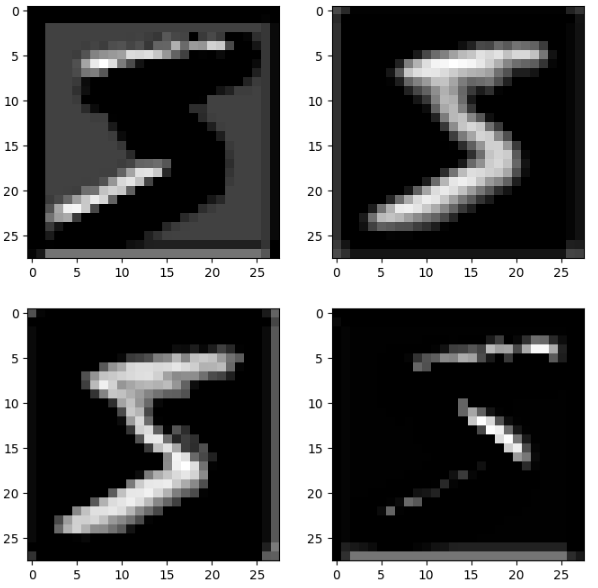
\includegraphics[width=1\linewidth]{Images/fpgac2.png}
        \caption{FPGA}
        \label{fig:enter-label}
    \end{subfigure}
    \begin{subfigure}[b]{0.45\linewidth}
        \includegraphics[width=1\linewidth]{Images/cnnc2.png}
        \caption{Tensorflow}
        \label{fig:enter-label}
        \end{subfigure}
    \caption{Ảnh ngõ ra lớp Conv2}
    \label{fig:main}
\end{figure}


\begin{figure}[H]
\centering
    \begin{subfigure}[b]{0.45\linewidth}
        \includegraphics[width=1\linewidth]{Images/fpgam1.png}
        \caption{FPGA}
        \label{fig:enter-label}
    \end{subfigure}
    \begin{subfigure}[b]{0.45\linewidth}
        \includegraphics[width=1\linewidth]{Images/cnnm1.png}
        \caption{Tensorflow}
        \label{fig:enter-label}
        \end{subfigure}
    \caption{Ảnh ngõ ra lớp Mpool1}
    \label{fig:main}
\end{figure}

\begin{figure}[H]
\centering
    \begin{subfigure}[b]{0.45\linewidth}
        \includegraphics[width=1\linewidth]{Images/fpgac3.png}
        \caption{FPGA}
        \label{fig:enter-label}
    \end{subfigure}
    \begin{subfigure}[b]{0.45\linewidth}
        \includegraphics[width=1\linewidth]{Images/cnnc3.png}
        \caption{Tensorflow}
        \label{fig:enter-label}
        \end{subfigure}
    \caption{Ảnh ngõ ra lớp Conv3}
    \label{fig:main}
    \end{figure}


\begin{figure}[H]
\centering
    \begin{subfigure}[b]{0.45\linewidth}
        \includegraphics[width=1\linewidth]{Images/fpgac4.png}
        \caption{FPGA}
        \label{fig:enter-label}
    \end{subfigure}
    \begin{subfigure}[b]{0.45\linewidth}
        \includegraphics[width=1\linewidth]{Images/cnnc4.png}
        \caption{Tensorflow}
        \label{fig:enter-label}
        \end{subfigure}
    \caption{Ảnh ngõ ra lớp Conv4}
    \label{fig:main}
\end{figure}


\begin{figure}[H]
\centering
    \begin{subfigure}[b]{0.45\linewidth}
        \includegraphics[width=1\linewidth]{Images/fpgam2.png}
        \caption{FPGA}
        \label{fig:enter-label}
    \end{subfigure}
    \begin{subfigure}[b]{0.45\linewidth}
        \includegraphics[width=1\linewidth]{Images/cnnm2.png}
        \caption{Tensorflow}
        \label{fig:enter-label}
        \end{subfigure}
    \caption{Ảnh ngõ ra lớp Mpool2}
    \label{fig:main}
\end{figure}


\begin{figure}[H]
\centering
    \begin{subfigure}[b]{0.45\linewidth}
        \includegraphics[width=1\linewidth]{Images/fpgac5.png}
        \caption{FPGA}
        \label{fig:enter-label}
    \end{subfigure}
    \begin{subfigure}[b]{0.45\linewidth}
        \includegraphics[width=1\linewidth]{Images/cnnc5.png}
        \caption{Tensorflow}
        \label{fig:enter-label}
        \end{subfigure}
    \caption{Ảnh ngõ ra lớp Conv5}
    \label{fig:main}
\end{figure}

\begin{figure}[H]
  \centering
    \begin{subfigure}[b]{\textwidth}
        \centering
        \includegraphics[width=0.75\linewidth]{Images/fpgagm.png}
        \caption{FPGA}
        \label{fig:enter-label}
    \end{subfigure}
    \vspace{1em} % Add vertical spacing
    \begin{subfigure}[b]{\textwidth}
        \centering
        \includegraphics[width=0.75\linewidth]{Images/cnngm.png}
        \caption{Tensorflow}
        \label{fig:enter-label}
    \end{subfigure}
    \caption{Kết quả ngõ ra Global max pooling}
\end{figure}
Ở kết quả ngõ ra Global max pooling có thể thấy kết quả 2 bên có phần chệnh lệch với nhau do các trọng số trên FPGA đã được lượng tử hóa nên sẽ có sai số lượng tử.

\begin{figure}[H]
    \centering
    \includegraphics[width=0.75\linewidth]{Images/Screenshot 2025-04-16 192852.png}
    \caption{Giả lập dự đoán tập dữ liệu test MNIST trên Xcelium}
    \label{fig:enter-label}
\end{figure}
Tiến hành test trên bộ dữ liệu Test-set MNIST ta thấy tỉ lệ dự đoán chính xác là 91.5\%, giảm 0.86\% so với mô hình Binary CNN ta tính toán trên máy tính là 92.36\% (Hình \ref{fig:mnisttest}) do ta lượng tử hóa các trọng số về kiểu dữ liệu số fixed-point Q4.8. Thời gian nhận diện 10000 ảnh là $70837499995ns$ với xung clock với chu kì $10ns$ vị chi ta tốn 708375 chu kì clock để nhận diện 1 ảnh. Nếu Module nhận diện số viết tay này sử dụng xung clock 10MHz ta sẽ tốn $\approx71ms$ để xử lí 1 ảnh.

\begin{center}
\begin{table}[H]
\centering
\caption{FPGA-based MNIST Recognition Models Comparison}
\label{tab:mnist_fpga_rotated}
\begin{tabular}{|p{2cm}|p{2cm}|p{2cm}|p{2cm}|p{2cm}|p{2cm}|p{2cm}|}
\hline
\textbf{Model Architecture} & \textbf{Binarized CNN (BNN)} & \textbf{8-bit Quantized CNN} & \textbf{3-Layer MLP} & \textbf{Pruned CNN (Winograd)} & \textbf{Spiking Neural Network} & \textbf{Hybrid CNN-SVM} \\ \hline
\textbf{FPGA Device} & Xilinx Zynq-7020 & Xilinx Virtex-7 & Intel Cyclone V & Xilinx Kintex-7 & Xilinx Spartan-6 & Xilinx Zynq UltraScale \\ \hline
\textbf{LUTs} & 4,500 & 120,000 & 2,300 & 85,000 & 6,200 & 65,000 \\ \hline
\textbf{Clock Cycles} & 30 & 50 & 100 & 20 & 500 & 70 \\ \hline
\textbf{Accuracy (\%)} & 96.4 & 99.1 & 92.0 & 98.5 & 89.7 & 98.8 \\ \hline
\textbf{Freq. (MHz)} & 200 & 150 & 100 & 250 & 50 & 180 \\ \hline
\textbf{Power (W)} & 1.5 & 4.2 & 0.8 & 3.0 & 0.5 & 2.5 \\ \hline
\textbf{Toolchain} & FINN & Vivado HLS & Quartus & Vitis AI & Verilog & PYNQ \\ \hline
\textbf{Year} & 2018 & 2020 & 2017 & 2021 & 2019 & 2022 \\ \hline
\textbf{Remarks} & Binary weights/activations; low power & High DSP usage (256 blocks); pipelined & Minimal resources; no DSP & Winograd transforms; 80\% pruned & Event-driven; ultra-low power & CNN + SVM classifier \\ \hline
\end{tabular}
\end{table}
\end{center}

So sánh model của đồ án này với các model MNIST FPGA khác thì còn nhiều mặt hạn chế như tốc độ xử lý và độ chính xác tuy nhiên cấu trúc của thiết kế đơn giản phù hợp cho việc nghiên cứu cách hoạt động của mạng CNN cũng như FPGA so với các kiến trúc được tạo tự động từ các tool HLS (High-Level Synthesis).

\subsection{Đưa lên kit thực tế}

Để kiểm tra hoạt động của thiết kế ở thực tế ta xây dựng hệ thống đơn giản bằng cách truyền dữ liệu ảnh xám 28x28 cần nhận diện qua UART module nhận diện chữ viết tay như hình \ref{fig:kit}.
\begin{figure}[H]
    \centering
    \includegraphics[width=1\linewidth]{Images/cnn_dut_mnist_test-Page-2.drawio.png}
    \caption{Sơ đồ khối hệ thống thực tế}
    \label{fig:kit}
\end{figure}

Với khối UART receiver ta thiết kế như lưu đồ sau.
\begin{figure}[H]
    \centering
    \includegraphics[width=0.5\linewidth]{Images/uartrx.png}
    \caption{UART receiver fsm}
    \label{fig:enter-label}
\end{figure}

Khối controller sẽ nhận các lệnh từ UART bao gồm lệnh load ảnh vào RAM \textit{(nhận kí tự "g")} và lệnh bắt đầu nhân diện số viết tay \textit{(nhận kí tự "d")}.
\begin{figure}[H]
    \centering
    \includegraphics[width=0.6\linewidth]{Images/controller_flow.png}
    \caption{Controller flow chart}
    \label{fig:enter-label}
\end{figure}

Khối LCD Driver có nhiệm vụ đọc dữ liệu ảnh từ RAM và điều khiển các tín hiệu quét ngang và dọc để đưa ảnh lên màn hình.
\begin{figure}[H]
    \centering
    \includegraphics[width=1\linewidth]{Images/lcdriver.png}
    \caption{LCD driver flow chart}
    \label{fig:enter-label}
\end{figure}

Ngoài ra ta cần viết thêm phần mềm đơn giản bằng python sử dung thư viện Tkinter để làm UI và Pyserial để giaop tiếp UART để gửi lệnh và dữ liệu ảnh số viết tay cần nhận diện và có thêm tính năng cho người dùng tự vẽ số viết tay để kiểm tra hoạt động của thiết kế.
\begin{figure}[H]
    \centering
    \includegraphics[width=1\linewidth]{Images/sw.png}
    \caption{Giao diện phần mềm}
    \label{fig:sw}
\end{figure}

Gửi hình ảnh số 2 trên phần mềm như hình \ref{fig:sw} và gửi lệnh nhận diện ta có kết quả ngõ ra hiển thị ngõ ra của khối CNN trên led của kit là 0100 và kết quả hiển thị trên led 7 đoạn là 2.
\begin{figure}[H]
    \centering
    \includegraphics[width=0.75\linewidth]{Images/testr.png}
    \caption{Kết quả nhận diện trên FPGA}
    \label{fig:enter-label}
\end{figure}

Bảng dưới đây là báo cáo tài nguyên mà hệ thống này sử dụng trên kit Tang Nano 9K.
\begin{table}[H]
\centering
\caption{Resource Utilization Summary}
\label{tab:resource_utilization_summary}
\begin{tabular}{l r@{\hspace{1em}}l S[table-format=2.1]}
\toprule
\multirow{2}{*}{\textbf{Resource}} & 
\multicolumn{2}{c}{\textbf{Used/Total}} & 
\multirow{2}{*}{\textbf{Utilization}} \\
& \multicolumn{2}{c}{(units)} & \\
\midrule
Logic & 3305 (1841 LUT, 1446 ALU, 3 RAM16) & / 8640 & 39.0\% \\
Register & 519 & / 6693 & 8.0\% \\
\quad $\bullet$ Register as Latch & 0 & / 6693 & 0.0\% \\
\quad $\bullet$ Register as FF & 519 & / 6693 & 8.0\% \\
BSRAM & 20 & / 26 & 77.0\% \\
\bottomrule
\end{tabular}
\end{table}

Với báo cáo timming với $F_{max}=15.733MHz$ trên kit Tang Nano 9K để cho dễ dàng canh thơi gian cho khung truyền UART ta chọn được tần số 10.8Mhz với baundrate 9600 vì 10.8Mhz chia hết cho 9600 thì UART sẽ truyền dữ liệu tốt nhất.
\begin{figure}[H]
    \centering
    \includegraphics[width=1\linewidth]{Images/timing.png}
    \caption{Báo cáo timming hệ thống}
    \label{fig:enter-label}
\end{figure}

\newpage
\section{ĐÁNH GIÁ CHUNG VÀ KẾT LUẬN}
Sau thời gian thực hiện đồ án, em có những đánh giá và kết luận chung sau khi hoàn thành như sau:
\begin{itemize}
    \item Về những kết quả thu được:
    \begin{itemize}
        \item \textbf{Thiết kế hệ thống phần cứng}: Đã thành thạo quy trình thiết kế hệ thống trên FPGA, bao gồm phân tích yêu cầu, chia module chức năng (LCD driver, UART controller, CNN) và triển khai bằng Verilog/SystemVerilog.
        \item \textbf{Mô phỏng và kiểm tra}: Làm chủ công cụ mô phỏng (ModelSim/Xcelium) để verify chức năng các module, phát hiện lỗi timing thông qua testbench tự động và phân tích waveform.
        \item \textbf{Nâng cao kỹ năng tích hợp}: Rèn luyện khả năng tích hợp đa module (kết hợp phần cứng-phần mềm), xử lý giao tiếp UART, điều khiển VGA và tối ưu hóa pipeline cho bộ suy luận CNN.
    \end{itemize}
    
    \item Về những hạn chế còn tồn đọng:
    \begin{itemize}

        \item \textbf{Thời gian xử lý}: Thời gian xử lý còn chậm so với các model cùng chức năng khác.
        \item \textbf{Tối ưu tài nguyên}: Chưa khai thác hiệu quả BRAM/DSP slices trên FPGA, dẫn đến lãng phí tài nguyên và hạn chế tốc độ xử lý.
        \item \textbf{Chưa xử lý lỗi thời gian thực}: Thiếu cơ chế phục hồi khi gặp lỗi giao tiếp UART hoặc mất đồng bộ tín hiệu VGA, gây treo hệ thống.
    \end{itemize}
\end{itemize}

Qua những đánh giá trên, bản thân đã:
\begin{itemize}
    \item[+] Tiếp thu sâu về kiến trúc FPGA và phương pháp thiết kế RTL
    \item[+] Phát triển tư duy hệ thống thông qua tích hợp đa thành phần
    \item[+] Nhận thức rõ tầm quan trọng của timing closure và power analysis
\end{itemize}

Tuy nhiên, cần khắc phục ngay:
\begin{itemize}
    \item[--] Bổ sung kỹ thuật timing constraints (SDC) để đảm bảo Fmax
    \item[--] Nâng cao kỹ năng debug bằng công cụ của tool và giả lập.
    \item[--] Xây dựng testbench coverage-driven cho các trường hợp biên
\end{itemize}

\newpage
\section{TÀI LIỆU THAM KHẢO}

\begin{thebibliography}{9999}
\bibitem{hubara2016binarized}
Hubara, I., Courbariaux, M., Soudry, D., \& El-Yaniv, R. (2016). "Binarized Neural Networks". \textit{Advances in Neural Information Processing Systems} (NIPS).

\bibitem{umuroglu2017finn}
Umuroglu, Y., et al. (2017). "FINN: A Framework for Fast, Scalable Binarized Neural Network Inference". \textit{ACM/SIGDA International Symposium on FPGAs}.

\bibitem{lecun1998gradient}
LeCun, Y., Bottou, L., Bengio, Y., \& Haffner, P. (1998). "Gradient-Based Learning Applied to Document Recognition". \textit{Proceedings of the IEEE}.


\bibitem{altera2024optimized}
Intel FPGA (2024). "Optimized CNN Acceleration for Cyclone V FPGAs". \textit{Intel White Paper WP-01234}.

\bibitem{rastegari2016xnor}
Rastegari, M., et al. (2016). "XNOR-Net: ImageNet Classification Using Binary Convolutional Neural Networks". \textit{European Conference on Computer Vision (ECCV)}.

\bibitem{mnist1998}
Yann LeCun \& Corinna Cortes. (1998). "The MNIST Database of Handwritten Digits". [Online]. Available: http://yann.lecun.com/exdb/mnist/

\bibitem{verilog2005standard}
IEEE Standard 1364-2005 (2005). \textit{IEEE Standard for Verilog Hardware Description Language}.
\end{thebibliography}

\end{document}